% !TeX spellcheck = es_MX
\documentclass[12pt, a4paper, titlepage]{article}
\usepackage[spanish]{babel}
\usepackage[utf8]{inputenc}
\usepackage[linesnumbered,lined,boxed,commentsnumbered]{algorithm2e}
\usepackage{enumitem,kantlipsum}
\usepackage{array}
\usepackage{placeins}
% Códigos y codificación para caracteres en español
\usepackage{listings}
\usepackage{color}
\lstset{literate=
	{á}{{\'a}}1 {é}{{\'e}}1 {í}{{\'i}}1 {ó}{{\'o}}1 {ú}{{\'u}}1
	{Á}{{\'A}}1 {É}{{\'E}}1 {Í}{{\'I}}1 {Ó}{{\'O}}1 {Ú}{{\'U}}1
	{à}{{\`a}}1 {è}{{\`e}}1 {ì}{{\`i}}1 {ò}{{\`o}}1 {ù}{{\`u}}1
	{À}{{\`A}}1 {È}{{\'E}}1 {Ì}{{\`I}}1 {Ò}{{\`O}}1 {Ù}{{\`U}}1
	{ä}{{\"a}}1 {ë}{{\"e}}1 {ï}{{\"i}}1 {ö}{{\"o}}1 {ü}{{\"u}}1
	{Ä}{{\"A}}1 {Ë}{{\"E}}1 {Ï}{{\"I}}1 {Ö}{{\"O}}1 {Ü}{{\"U}}1
	{â}{{\^a}}1 {ê}{{\^e}}1 {î}{{\^i}}1 {ô}{{\^o}}1 {û}{{\^u}}1
	{Â}{{\^A}}1 {Ê}{{\^E}}1 {Î}{{\^I}}1 {Ô}{{\^O}}1 {Û}{{\^U}}1
	{œ}{{\oe}}1 {Œ}{{\OE}}1 {æ}{{\ae}}1 {Æ}{{\AE}}1 {ß}{{\ss}}1
	{ű}{{\H{u}}}1 {Ű}{{\H{U}}}1 {ő}{{\H{o}}}1 {Ő}{{\H{O}}}1
	{ç}{{\c c}}1 {Ç}{{\c C}}1 {ø}{{\o}}1 {å}{{\r a}}1 {Å}{{\r A}}1
	{€}{{\EUR}}1 {£}{{\pounds}}1
}
%%Appendix
\usepackage[toc,page]{appendix}

%%Tablas
\usepackage{tabularx}

%%otros
\usepackage{float}
\usepackage{subfig}
\usepackage{comment}

% http://ctan.org/pkg/booktabs
\usepackage{booktabs}
\newcommand{\tabitem}{~~\llap{\textbullet}~~}

%%Imágenes
\usepackage{graphicx}

%%Colores de texto 
\usepackage{xcolor}
\usepackage{colortbl}

%%Links
\usepackage[hidelinks]{hyperref}

%%Comentarios
\usepackage{verbatim}

%%PARA IMÁGENES EN LÍNEA
%\usepackage[english]{babel}

%%Acrónimos
\usepackage[acronym]{glossaries}

%%Glosario
\usepackage{glossaries}

\usepackage{pdfpages}

%%ESTILO DE CÓDIGO
\lstdefinestyle{codeStyle}{
	backgroundcolor=\color{backcolour}, commentstyle=\color{commentcolor},
	keywordstyle=\color{guindapoli},
	numberstyle=\tiny\color{azulescom},
	stringstyle=\color{azulfuerte},
	basicstyle=\ttfamily\footnotesize,
	breakatwhitespace=false, 
	breaklines=true, 
	captionpos=b,
	keepspaces=true,
	numbers=left,
	numbersep=5pt,
	showspaces=false,
	showstringspaces=false,
	showtabs=false,
	tabsize=3
}
\definecolor{delim}{RGB}{20,105,176}

%% CENTRADO VERTICAL
\newcolumntype{M}[1]{>{\centering\arraybackslash}m{#1}}

%% CENTRADO HORIZONTAL
\newcolumntype{P}[1]{>{\centering\arraybackslash}p{#1}}

%% JSON
\lstdefinelanguage{json}{
	basicstyle=\normalfont\ttfamily,
	numbers=left,
	numberstyle=\tiny\color{azulescom},
	stringstyle=\color{azulfuerte},
	stepnumber=1,
	numbersep=8pt,
	showstringspaces=false,
	breaklines=true,
	backgroundcolor=\color{backcolour},
	literate=
	*{0}{{{\color{azulfuerte}0}}}{1}
	{1}{{{\color{azulfuerte}1}}}{1}
	{2}{{{\color{azulfuerte}2}}}{1}
	{3}{{{\color{azulfuerte}3}}}{1}
	{4}{{{\color{azulfuerte}4}}}{1}
	{5}{{{\color{azulfuerte}5}}}{1}
	{6}{{{\color{azulfuerte}6}}}{1}
	{7}{{{\color{azulfuerte}7}}}{1}
	{8}{{{\color{azulfuerte}8}}}{1}
	{9}{{{\color{azulfuerte}9}}}{1}
	{:}{{{\color{guindapoli}{:}}}}{1}
	{,}{{{\color{guindapoli}{,}}}}{1}
	{\{}{{{\color{guindapoli}{\{}}}}{1}
	{\}}{{{\color{guindapoli}{\}}}}}{1}
	{[}{{{\color{guindapoli}{[}}}}{1}
	{]}{{{\color{guindapoli}{]}}}}{1},
}

\lstset{style=codeStyle}


\definecolor{lightgray}{rgb}{.9,.9,.9}
\definecolor{darkgray}{rgb}{.4,.4,.4}
\definecolor{purple}{rgb}{0.65, 0.12, 0.82}

%% Javascript
\lstdefinelanguage{JavaScript}{
	keywords={typeof, new, true, false, catch, function, return, null, catch, switch, var, if, in, while, do, else, case, break, let, continue},
	keywordstyle=\color{blue}\bfseries,
	ndkeywords={class, export, boolean, throw, implements, import, this},
	ndkeywordstyle=\color{darkgray}\bfseries,
	identifierstyle=\color{black},
	sensitive=false,
	comment=[l]{//},
	morecomment=[s]{/*}{*/},
	commentstyle=\color{purple}\ttfamily,
	stringstyle=\color{red}\ttfamily,
	morestring=[b]',
	morestring=[b]"
}

\lstset{
	language=JavaScript,
	backgroundcolor=\color{lightgray},
	extendedchars=true,
	basicstyle=\footnotesize\ttfamily,
	showstringspaces=false,
	showspaces=false,
	numbers=left,
	numberstyle=\footnotesize,
	numbersep=9pt,
	tabsize=2,
	breaklines=true,
	showtabs=false,
	captionpos=b
}
%% ESTO ES PYTHON

\definecolor{maroon}{cmyk}{0, 0.87, 0.68, 0.32}
\definecolor{halfgray}{gray}{0.55}
\definecolor{ipython_frame}{RGB}{207, 207, 207}
\definecolor{ipython_bg}{RGB}{247, 247, 247}
\definecolor{ipython_red}{RGB}{186, 33, 33}
\definecolor{ipython_green}{RGB}{0, 128, 0}
\definecolor{ipython_cyan}{RGB}{64, 128, 128}
\definecolor{ipython_purple}{RGB}{170, 34, 255}

\lstset{
	breaklines=true,
	extendedchars=true,
	literate=
	{á}{{\'a}}1 {é}{{\'e}}1 {í}{{\'i}}1 {ó}{{\'o}}1 {ú}{{\'u}}1
	{Á}{{\'A}}1 {É}{{\'E}}1 {Í}{{\'I}}1 {Ó}{{\'O}}1 {Ú}{{\'U}}1
	{à}{{\`a}}1 {è}{{\`e}}1 {ì}{{\`i}}1 {ò}{{\`o}}1 {ù}{{\`u}}1
	{À}{{\`A}}1 {È}{{\'E}}1 {Ì}{{\`I}}1 {Ò}{{\`O}}1 {Ù}{{\`U}}1
	{ä}{{\"a}}1 {ë}{{\"e}}1 {ï}{{\"i}}1 {ö}{{\"o}}1 {ü}{{\"u}}1
	{Ä}{{\"A}}1 {Ë}{{\"E}}1 {Ï}{{\"I}}1 {Ö}{{\"O}}1 {Ü}{{\"U}}1
	{â}{{\^a}}1 {ê}{{\^e}}1 {î}{{\^i}}1 {ô}{{\^o}}1 {û}{{\^u}}1
	{Â}{{\^A}}1 {Ê}{{\^E}}1 {Î}{{\^I}}1 {Ô}{{\^O}}1 {Û}{{\^U}}1
	{œ}{{\oe}}1 {Œ}{{\OE}}1 {æ}{{\ae}}1 {Æ}{{\AE}}1 {ß}{{\ss}}1
	{ç}{{\c c}}1 {Ç}{{\c C}}1 {ø}{{\o}}1 {å}{{\r a}}1 {Å}{{\r A}}1
	{€}{{\EUR}}1 {£}{{\pounds}}1
}

\lstdefinelanguage{python}{
	morekeywords={access,and,break,class,continue,def,del,elif,else,except,exec,finally,for,from,global,if,import,in,is,lambda,not,or,pass,print,raise,return,try,while},
	morekeywords=[2]{abs,all,any,basestring,bin,bool,bytearray,callable,chr,classmethod,cmp,compile,complex,delattr,dict,dir,divmod,enumerate,eval,execfile,file,filter,float,format,frozenset,getattr,globals,hasattr,hash,help,hex,id,input,int,isinstance,issubclass,iter,len,list,locals,long,map,max,memoryview,min,next,object,oct,open,ord,pow,property,range,raw_input,reduce,reload,repr,reversed,round,set,setattr,slice,sorted,staticmethod,str,sum,super,tuple,type,unichr,unicode,vars,xrange,zip,apply,buffer,coerce,intern},
	sensitive=true,
	morecomment=[l]\#,
	morestring=[b]',
	morestring=[b]",
	morestring=[s]{'''}{'''},
	morestring=[s]{"""}{"""},
	morestring=[s]{r'}{'},
	morestring=[s]{r"}{"},
	morestring=[s]{r'''}{'''},
	morestring=[s]{r"""}{"""},
	morestring=[s]{u'}{'},
	morestring=[s]{u"}{"},
	morestring=[s]{u'''}{'''},
	morestring=[s]{u"""}{"""},
	% {replace}{replacement}{lenght of replace}
	% *{-}{-}{1} will not replace in comments and so on
	literate=
	{á}{{\'a}}1 {é}{{\'e}}1 {í}{{\'i}}1 {ó}{{\'o}}1 {ú}{{\'u}}1
	{Á}{{\'A}}1 {É}{{\'E}}1 {Í}{{\'I}}1 {Ó}{{\'O}}1 {Ú}{{\'U}}1
	{à}{{\`a}}1 {è}{{\`e}}1 {ì}{{\`i}}1 {ò}{{\`o}}1 {ù}{{\`u}}1
	{À}{{\`A}}1 {È}{{\'E}}1 {Ì}{{\`I}}1 {Ò}{{\`O}}1 {Ù}{{\`U}}1
	{ä}{{\"a}}1 {ë}{{\"e}}1 {ï}{{\"i}}1 {ö}{{\"o}}1 {ü}{{\"u}}1
	{Ä}{{\"A}}1 {Ë}{{\"E}}1 {Ï}{{\"I}}1 {Ö}{{\"O}}1 {Ü}{{\"U}}1
	{â}{{\^a}}1 {ê}{{\^e}}1 {î}{{\^i}}1 {ô}{{\^o}}1 {û}{{\^u}}1
	{Â}{{\^A}}1 {Ê}{{\^E}}1 {Î}{{\^I}}1 {Ô}{{\^O}}1 {Û}{{\^U}}1
	{œ}{{\oe}}1 {Œ}{{\OE}}1 {æ}{{\ae}}1 {Æ}{{\AE}}1 {ß}{{\ss}}1
	{ç}{{\c c}}1 {Ç}{{\c C}}1 {ø}{{\o}}1 {å}{{\r a}}1 {Å}{{\r A}}1
	{€}{{\EUR}}1 {£}{{\pounds}}1
	%
	{^}{{{\color{ipython_purple}\^{}}}}1
	{=}{{{\color{ipython_purple}=}}}1
	%
	{+}{{{\color{ipython_purple}+}}}1
	{*}{{{\color{ipython_purple}$^\ast$}}}1
	{/}{{{\color{ipython_purple}/}}}1
	%
	{+=}{{{+=}}}1
	{-=}{{{-=}}}1
	{*=}{{{$^\ast$=}}}1
	{/=}{{{/=}}}1,
	literate=
	*{-}{{{\color{ipython_purple}-}}}1
	{?}{{{\color{ipython_purple}?}}}1,
	%
	identifierstyle=\color{black}\ttfamily,
	commentstyle=\color{ipython_cyan}\ttfamily,
	stringstyle=\color{ipython_red}\ttfamily,
	keepspaces=true,
	showspaces=false,
	showstringspaces=false,
	rulecolor=\color{ipython_frame},
	frame=single,
	frameround={t}{t}{t}{t},
	framexleftmargin=6mm,
	numbers=left,
	numberstyle=\tiny\color{halfgray},
	backgroundcolor=\color{ipython_bg},
	% extendedchars=true,
	basicstyle=\scriptsize,
	keywordstyle=\color{ipython_green}\ttfamily,
}
%------------------------------------------------ESTABLECER COLORES------------------------------------------------%

\definecolor{guindapoli}{RGB}{102, 0, 51}
\definecolor{azulescom}{RGB}{0, 0, 102}
\definecolor{azulclaro}{RGB}{222, 232, 255}
\definecolor{azulfuerte}{RGB}{60, 150, 250}

%------------------------------------------------COLORES PARA CÓDIGO------------------------------------------------%

\definecolor{commentcolor}{RGB}{ 192, 192, 192 }
\definecolor{backcolour}{RGB}{ 249, 249, 249 }

%------------------------------------------------FIN DE COLORES------------------------------------------------%

%------------------------------------------------ACRÓNIMOS------------------------------------------------%

\newacronym{mvc}{MVC}{Modelo-Vista-Controlador}
\newacronym{orm}{ORM}{Object Relational Manager}
\newacronym{wsgi}{WSGI}{Web Server Gateway Interface}
\newacronym{dbms}{DBMS}{Sistema de gestión de base de datos}
\newacronym{bert}{BERT}{Bidirectional Encoder Representations from Transformers}
\newacronym{pln}{PLN}{Procesamiento del Lenguaje Natural}
\newacronym{mlm}{MLM}{Modelado de Lenguaje Enmascarado}
\newacronym{gpt}{GPT}{Generative Pretrained Transformer}
\newacronym{bpe}{BPE}{Byte Pair Encoding}
\newacronym{wip}{WIP}{Work In Progress}
\newacronym{cls}{CLS}{Classification}
\newacronym{sep}{SEP}{Separate}
\newacronym{json}{JSON}{Javascript Object Notation}
\newacronym{url}{URL}{Uniform Source Locator}
\newacronym{http}{HTTP}{Hypertext Transfer Protocol}
\newacronym{tcp}{TCP}{Transmission Control Protocol}
\newacronym{udp}{UDP}{User Datagram Protocol}
\newacronym{imap}{IMAP}{Internet Message Access Protocol}
\newacronym{pop}{POP}{Post Office Protocol}
\newacronym{smtp}{SMTP}{Simple Mail Transfer Protocol}
\newacronym{vps}{VPS}{Virtual Private Server}
\newacronym{ssl}{SSL}{Secure Socket Layer}
\newacronym{fqdn}{FQDN}{Fully Qualified Domain Name}
\newacronym{aws}{AWS}{Amazon Web Services}
\newacronym{gpu}{GPU}{Graphic Processor Unit}
\newacronym{ec2}{EC2}{Elastic Compute Cloud}
\newacronym{ui}{UI}{User Interface}
\newacronym{api}{API}{Application Programm Interface}
\newacronym{gcp}{GCP}{Google Cloud Platform}
\newacronym{sdk}{SDK}{Software Development Kit}
\newacronym{html}{HTML}{Hypertext Markup Language}
\newacronym{css}{CSS}{Cascading Style Sheet}
\newacronym{ecma}{ECMA}{European Computer Manufacturers Association}
\newacronym{https}{HTTPS}{Hypertext Transfer Protocol Secure}
\newacronym{tls}{TLS}{Transport Layer Security}
\newacronym{sql}{SQL}{Structured Query Language}
\newacronym{cad}{CAD}{Computer Aided Design}
\newacronym{cli}{CLI}{Command Line Interface}
\newacronym{s3}{S3}{Simple Storage Service}
\newacronym{hdd}{HDD}{Hard Drive Disk}
\newacronym{ssd}{SSD}{Solid State Drive}
\newacronym{iso}{ISO}{International Standardization Organization}
\newacronym{xml}{XML}{Extensible Markup Language}
\newacronym{svg}{SVG}{Scalable Vector Graphics}
\newacronym{rnn}{RNN}{Recurrent Neural Network}
\newacronym{lstm}{LSTM}{Long Short Term Memory}
%------------------------------------------------FINAL DE ACRÓNIMOS------------------------------------------------%

\begin{document}
	%%PARA QUE DETECTE HASTA SUBSUBSECTION
	\setcounter{secnumdepth}{3}
	
	%%%%%%%%%%%%%%%%%%%%%%%%%%%%%%%%%%%%%%%%%%%%%%%%%%%%%%%%%
	%                                                       																																		  %
	%                                                      																																	  		  %
	%              																	PORTADA  																				  			 %
	%                                                      																																			  %
	%                                                      																																			  %
	%%%%%%%%%%%%%%%%%%%%%%%%%%%%%%%%%%%%%%%%%%%%%%%%%%%%%%%%%
	\begin{titlepage}	
		
		\newcommand{\HRule}{\rule{\linewidth}{0.5mm}}									%%%\left
		%%%
		\begin{minipage}{0.48\textwidth} \begin{flushleft}
				
\includegraphics[scale = 0.10]{Imagenes/Logos/logoescom.png}
		\end{flushleft}\end{minipage}
		\begin{minipage}{0.48\textwidth} \begin{flushright}
				
\includegraphics[scale = 0.55]{Imagenes/Logos/logoipn.png}
		\end{flushright}\end{minipage}
		
		%%%
		\vspace*{.25cm}								%%%
		
		\begin{center}
			
			\begin{LARGE}
				\textcolor{guindapoli}{INSTITUTO POLITÉCNICO NACIONAL}\\
			\end{LARGE}	
			
			\vspace*{0.2in}
			
			\begin{Large}
				\textcolor{azulescom}{ESCUELA SUPERIOR DE CÓMPUTO}\\
			\end{Large}	
			
			\vspace*{0.4in}
			
			\begin{large}
				Manual Técnico\\
			\end{large}	
			
			\vspace*{0.4in}
			
			\begin{large}
				Trabajo Terminal TT2020-B002\\
			\end{large}
			
			\vspace*{0.2in}
			
			\begin{Large}
				\textbf{Generador de versos musicales en el idioma
					inglés por medio de procesamiento de lenguaje
					natural y redes neuronales}\\
			\end{Large}
			
			\vspace*{0.2in}
			
			\rule{80mm}{.1mm}\\
			\vspace*{0.1in}
			
			\begin{large}
				\begin{center}
					\textbf{Presentan}:\\
					Espinosa de los Monteros Lechuga Jaime Daniel\\
					Nava Romo Edgar Adrián\\
					Salgado Gómez Alfredo Emilio\\
				\end{center}
			\end{large}
			
			\begin{large}
				\textbf{Directores}:\\
				Olga Kolesnikova\\
				Ariel López Rojas\\
			\end{large}
			
		\end{center}
		
	\end{titlepage}
	
	%%%%%%%%%%%%%%%%%%%%%%%%%%%%%%%%%%%%%%%%%%%%%%%%%%%%%%%%%
	%                                                       																																		  %
	%                                                      																																	  		  %
	%              																	 ÍNDICE  																				  			 	  %
	%                                                      																																			  %
	%                                                      																																			  %
	%%%%%%%%%%%%%%%%%%%%%%%%%%%%%%%%%%%%%%%%%%%%%%%%%%%%%%%%%
	% Firma directores
	\newpage
	\section*{Firmas de Directores}
	
	\vfill  % push the rest to the bottom of the page
	\noindent 
	\parbox[b]{0.4\linewidth}{% size of the first signature box
		\strut 
		Firmado por: \\[3cm]% This 2cm is the space for the signature under the names
		\hrule
		Profesor: Ariel López Rojas} 
	\hspace{1cm} % distance between the two signature blocks 
	\parbox[b]{0.4\linewidth}{% ...and the second one
		\strut 
		\\[3cm]% This 2cm is the space for the signature under the names
		\hrule
		Doctora Olga Kolesnikova} 
	\par\vspace{1cm} 
	\newpage
	% Rename Appendice to Anexos
	\renewcommand\appendixpagename{Índice}
	\renewcommand\appendixtocname{Índice}
	\appendixpageoff
	\begin{appendices}
		\renewcommand*\contentsname{{\textcolor{azulescom}{Índice.}}}
		\tableofcontents
		\newpage
		%%índice de figuras
		\renewcommand*\listfigurename{{\textcolor{azulescom}{Índice de figuras.}}}
		\listoffigures
		\newpage
		%%Índice de tablas
		\newpage
		\renewcommand*\listtablename{{\textcolor{azulescom}{Índice de cuadros.}}}
		\listoftables
		\newpage
	\end{appendices}
	
	\section{Presentación}
	El presente manual se ha desarrollado con el objetivo de dar a conocer la información necesaria requerida por quien llegue a dar soporte a la aplicación web. La intención es proporcionar detalles, en un mayor desglose, de los requerimientos seguidos para su elaboración, así como del desarrollo de la aplicación web, la generación del modelo, la conexión entre la aplicación web y el modelo, las herramientas empleadas y la funcionalidad final.
	\section{Resumen}
	El manual detalla los aspectos técnicos e informáticos relacionados con el desarrollo de la aplicación web y la finalidad es dar a conocer información necesaria para su manejo u operación al personal que vaya a administrarlo, modificarlo o que tenga como intención el darle mantenimiento, así mismo se exponen en mayor detalle las herramientas utilizadas para su desarrollo.
	\newpage
	\section{Introducción}
	El manual describe los pasos requeridos que deben de seguirse para que cualquier operador con nociones básicas de sistemas computacionales pueda administrar, editar o configurar la aplicación web de tal manera que el sistema responda de una manera adecuada y acorde a lo esperado.\\\\
	Se presentan las herramientas utilizadas para el desarrollo de la aplicación web, así como los pasos que fueron necesarios para la configuración y despliegue de la misma haciendo uso de diagramas e ilustraciones alusivas al funcionamiento como una forma de apoyo visual; se detallan los requerimientos mínimos de hardware y software requeridos para el correcto desempeño de la aplicación web.
	\section{Objetivo}
	Dar a conocer al usuario la estructura de la aplicación web y la forma en la cual está conformada con la finalidad de que pueda darle soporte, realizar modificaciones o hacer actualizaciones a la misma.
	\newpage
	\section{Requerimientos mínimos técnicos}
	\subsection{Requisitos de hardware de aplicaciones web}
	En la siguiente tabla se enumeran los requisitos mínimos de hardware recomendados para el correcto desempeño de la aplicación web.
	
	\begin{table}[!htbp]
		\caption[Requisitos hardware]{Requisitos mínimos recomendados de hardware}
		\begin{tabular}{| M{4cm} | M{4cm} | M{4cm} |} 
			\hline
			\textbf{Componente} & \textbf{Mínimo} & \textbf{Recomendado} \\ 
			\hline
			Procesador & Procesador de x86 o x64 bits de doble núcleo de 1,9 gigahercios (GHz) o más con el conjunto de instrucciones SSE2 & Procesador de 64 bits de doble núcleo de 3,3 gigahercios (GHz) o más con el conjunto de instrucciones SSE2 \\ 
			\hline
			Memoria & 2 GB de RAM & 4 GB de RAM o más \\
			\hline
			Resolución  & Súper VGA con una resolución de 1024 x 768 & Súper VGA con una resolución de 1024 x 768 \\
			\hline
		\end{tabular}
	\end{table}
	
	La ejecución de la aplicación web en un equipo que no cumpla los requisitos recomendados puede producir un rendimiento inadecuado o no satisfactorio, y de no cumplir con los mínimos puede incluso llevar a un estado de error o de no ejecución.\\
	Haciendo uso del hardware adecuado (superior o igual al recomendado) se podrá percibir un rendimiento satisfactorio y agradable de la aplicación web, esto es, por ejemplo, un sistema con un procesador moderno de cuatro núcleos, velocidad de reloj más baja y más RAM.
	
	\subsection{Requisitos de red}
	La aplicación web fue diseñada de tal manera que funciona mejor en redes que cuentan con las siguientes características:
	
	\begin{itemize}
		\item Ancho de banda superior a 50 KBps (400 kbps)
		\item Latencia inferior a 150 ms
	\end{itemize}
	
	Hay que tener en cuenta que estos valores son los recomendados y no garantizan un rendimiento satisfactorio. Los valores sugeridos se tomaron de ejemplos de sistemas que usan solicitudes de un formulario con palabras recurrentes por lo que el resultado podría variar.
	
	\section{Herramientas utilizadas para el desarrollo}
	\subsection{Python}
	Python es un lenguaje de programación orientado a objetos, de alto nivel con semántica dinámica. Sus estructuras de datos integradas de alto nivel, combinadas con el tipado y enlace dinámico, lo hacen muy atractivo para el desarrollo rápido de aplicaciones, así como para su uso en scripts o para conectar componentes ya existentes. La sintaxis simple y fácil de aprender de Python enfatiza la legibilidad y, por lo tanto, reduce el costo de mantenimiento del programa. Python admite módulos y paquetes, lo que fomenta la modularidad del programa y la reutilización del código. \cite{refQuesPython}
	\subsection{HTML}
	\acrfull{html} es un lenguaje de marcado que define la estructura de una página web y su contenido. \acrshort{html} consta de una serie de elementos que se utilizan para encerrar o envolver diferentes partes del contenido para que estos se visualicen o actúen de cierta manera. Las etiquetas adjuntas pueden hacer que una palabra o imagen sea un hipervínculo a otro lugar, pueden poner palabras en cursiva, hacer que la fuente sea más grande o pequeña, etc. \cite{refHtml} \\\\\
	\acrshort{html}5 es la versión más reciente de HTML, la cual integra nuevos elementos, atributos y comportamientos. Permite describir de mejor manera el contenido de la página web, así como mejora su conectividad con el servidor y almacenamiento, posibilita que las páginas web puedan operar sin conexión usando los datos almacenados localmente del lado del cliente, otorga un mejor soporte al contenido multimedia, así como una mejor integración a API's y un mejor diseño usando \acrshort{css}3.	\cite{refHtml2}
	\subsection{CSS}
	\acrfull{css} es el lenguaje para describir la presentación de las páginas web, así como hacerlas más atractivas. Permite adaptar la presentación a diferentes tipos de dispositivos. \acrshort{css} es independiente de \acrshort{html} y puede ser empleado con cualquier otro lenguaje de marcado basado en \acrshort{xml} o \acrshort{svg}. Usando CSS se pueden controlar con precisión cómo se ven los elementos \acrshort{html} en el navegador, que presentará para las etiquetas de marcado el diseño que cada uno desee. La separación de \acrshort{html} de \acrshort{css} facilita el mantenimiento de los sitios, compartir las hojas de estilo entre páginas y adaptarlas a distintos ámbitos. \cite{refcss}\\\\
	Es un lenguaje basado en reglas: cada usuario define las reglas que especifican los grupos de estilos que van a aplicarse a elementos particulares o grupos de elementos de la página web.\\\\
	Antes de CSS, las etiquetas como fuente, color, estilo de fondo, alineación, borde y tamaño tenían que repetirse en cada elemento de una página web. Ahora con los CSS, podemos definir cómo se van a comportar las etiquetas, al ser guardado en un archivo por separado, esta misma configuración puede usarse en otra página web ahorrando tiempo diseñándola. Además de que CSS provee de mejor y más detallados atributos para cada etiqueta.
	\subsection{JavaScript}
	JavaScript es un lenguaje de programación o secuencias de comandos que permite implementar funciones complejas en las páginas web. Estos scripts pueden ser desarrollados en el mismo \acrshort{html} para que sean ejecutados automáticamente cuando se carga dicha páginas web, estos scripts se proporcionan y ejecutan como texto sin formato. No necesitan una preparación especial ni una compilación para ejecutarse. \cite{refjs}\\\\
	JavaScript puede ejecutarse no solo en un navegador, sino también en un servidor, o en cualquier dispositivo que tenga un programa especial llamado JavaScript engine, el cual permite interpretar y ejecutar los scripts.\\\\
	JavaScript permite crear contenido dinámico dentro de las páginas web, reaccionar ante algunas acciones realizadas por los usuarios como lo son los clics del ratón, el movimiento del puntero o el presionar cierta tecla, permite enviar peticiones al servidor, así como descargar y subir archivos, además es posible obtener y configurar cookies, mostrar mensajes o alertas al usuario.
	\subsection{Flask}
	Flask es un mini marco (framework) web, esto es, un módulo de Python el cual permite desarrollar aplicaciones web. No cuenta con un Manejador de Objetos Relacionales u \acrshort{orm} por sus siglas en inglés, pero si cuenta con características como el enrutamiento de \acrshort{url}S y un motor de plantillas. En general es un marco de aplicación web \acrshort{wsgi}.\\\\
	La \acrfull{wsgi} es una especificación que describe cómo se va a comunicar un servidor web con una aplicación web, y como se pueden llegar a enlazar distintas aplicaciones web para procesar una solicitud o una petición.
	\subsection{Gunicorn}
	Gunicorn, también conocido como unicornio verde “Green Unicorn”, es una de las muchas implementaciones de un \acrfull{wsgi} y se usa comúnmente para ejecutar aplicaciones web hechas con Python. Esta implemente la especificación \acrshort{wsgi} de frameworks como Django, Flask o Bottle.
	\subsection{Amazon EC2}	
	Amazon \acrfull{ec2} \cite{amazon_ec2} proporciona una infraestructura de tecnologías de información que se ejecuta en la nube y funciona como un centro de datos que se ejecuta en su propia sede. Es ideal para empresas que necesitan rendimiento, flexibilidad y potencia al mismo tiempo.\\\\
	Amazon \acrshort{ec2} es un servicio que permite alquilar un servidor o máquina virtual de forma remota para ejecutar aplicaciones.
	\subsection{Amazon Elastic Beanstalk}	
	Amazon Elastic Beanstalk \cite{amazon_elastic_beanstalk} es un servicio para implementar y escalar servicios y aplicaciones web con diferentes lenguajes de programación, para este proyecto será útil directamente para la administración de la API, entre las ventajas que se tienen en esta herramienta son el control total de los recursos, tiene una administración de escalamiento de acuerdo a las peticiones y recursos necesarios, la infraestructura detecta automáticamente la última versión y la corre por su cuenta y la implementación general es muy sencilla.
	\begin{comment}	
		\subsection{Amazon SageMaker}
		Amazon SageMaker \cite{amazon_sagemaker} es un servicio que ayuda a científicos y desarrolladores a construir, entrenar e implementar de manera rápida y sencilla modelos de machine learning.\\\\
		Para construir el modelo, este servicio cuenta con algoritmos de machine learning más utilizados que vienen preinstalados. También está preconfigurado para que pueda ejecutar Apache MXNet y TensorFlow.\\\\
		Para el entrenamiento, con un solo clic en la consola de servicio, es fácil comenzar a entrenar su modelo. Amazon SageMaker se encarga de cada infraestructura y facilita la escalabilidad. lo que permite entrenar los modelos a escala de peta-bytes Si se desea acelerar y simplificar el proceso de entrenamiento, se puede ajustar automáticamente el modelo para obtener la mejor precisión.\\\\
		Para desplegar el modelo entrenado, se aloja en un clúster de escalado automático de Amazon \acrshort{ec2}.
	\end{comment}	
	\subsection{Amazon S3}
	Amazon \acrfull{s3} \cite{amazon_s3}, como su nombre lo indica, es un servicio web proporcionado por \acrfull{aws} que proporciona almacenamiento altamente escalable en la nube.
	\newpage
	\section{Diagramas de la aplicación web}
	\subsection{Diagrama de casos de uso}
	En el diagrama de casos de uso se detalla el papel que desempeña la aplicación web con el usuario y con el servidor.	
	\begin{figure}[H] 
		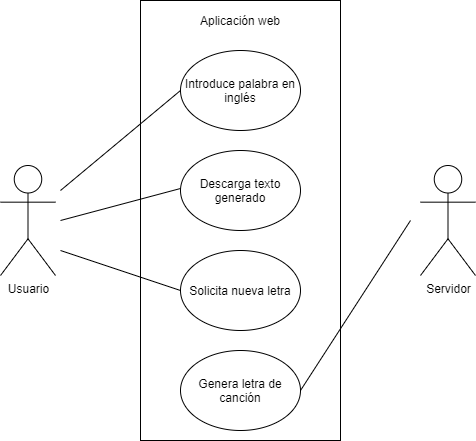
\includegraphics[width=13.5cm]{./Imagenes/Diagramas/CasoUso.png}
		\centering \caption{Diagrama de casos de uso}
	\end{figure}
	\newpage
	\begin{table}[hbt!]\caption{Caso de uso 1}% title of Table
		\centering % used for centering table
		\resizebox{13.5cm}{!} {
			\begin{tabular}{|c|c|}% centered columns (3 columns)
				\hline                        %inserts double horizontal lines
				\begin{tabular}[c]{@{}l@{}}Caso de uso\end{tabular}
				& \begin{tabular}[c]{@{}l@{}}Introducción de palabra en inglés\end{tabular} \\% inserting body of the table 
				\hline				                     
				\begin{tabular}[c]{@{}l@{}}Actores\end{tabular}
				& \begin{tabular}[c]{@{}l@{}}Usuario\end{tabular} \\% inserting body of the table 
				\hline
				\begin{tabular}[c]{@{}l@{}}Descripción\end{tabular}
				& \begin{tabular}[c]{@{}l@{}}El usuario dentro de la aplicación web proporciona una palabra\\ en el idioma inglés con la finalidad de generar un texto. \end{tabular} \\
				\hline
			\end{tabular}\label{table:Caso de uso 1}% is used to refer this table in the text
		}
	\end{table}
	\begin{table}[hbt!]\caption{Caso de uso 2}% title of Table
		\centering % used for centering table
		\resizebox{13.5cm}{!} {
			\begin{tabular}{|c|c|}% centered columns (3 columns)
				\hline                        %inserts double horizontal lines
				\begin{tabular}[c]{@{}l@{}}Caso de uso\end{tabular}
				& \begin{tabular}[c]{@{}l@{}}Descargar texto generado\end{tabular} \\% inserting body of the table 
				\hline				                     
				\begin{tabular}[c]{@{}l@{}}Actores\end{tabular}
				& \begin{tabular}[c]{@{}l@{}}Usuario\end{tabular} \\% inserting body of the table 
				\hline
				\begin{tabular}[c]{@{}l@{}}Descripción\end{tabular}
				& \begin{tabular}[c]{@{}l@{}}El usuario dentro de la aplicación web tiene la posibilidad\\ de descargar el texto generado por el modelo.  \end{tabular} \\
				\hline
			\end{tabular}\label{table:Caso de uso 2}% is used to refer this table in the text
		}
	\end{table}	
	\begin{table}[hbt!]\caption{Caso de uso 3}% title of Table
		\centering % used for centering table
		\resizebox{13.5cm}{!} {
			\begin{tabular}{|c|c|}% centered columns (3 columns)
				\hline                        %inserts double horizontal lines
				\begin{tabular}[c]{@{}l@{}}Caso de uso\end{tabular}
				& \begin{tabular}[c]{@{}l@{}}Solicitar nueva letra\end{tabular} \\% inserting body of the table 
				\hline				                     
				\begin{tabular}[c]{@{}l@{}}Actores\end{tabular}
				& \begin{tabular}[c]{@{}l@{}}Usuario\end{tabular} \\% inserting body of the table 
				\hline
				\begin{tabular}[c]{@{}l@{}}Descripción\end{tabular}
				& \begin{tabular}[c]{@{}l@{}}Al usuario dentro de la aplicación web se le da la posibilidad de volver\\ a generar otra letra musical haciendo uso de la misma palabra que \\proporcionó o utilizando una nueva.\end{tabular} \\
				\hline
			\end{tabular}\label{table:Caso de uso 3}% is used to refer this table in the text
		}
	\end{table}	
	\begin{table}[hbt!]\caption{Caso de uso 4}% title of Table
		\centering % used for centering table
		\resizebox{13.5cm}{!} {
			\begin{tabular}{|c|c|}% centered columns (3 columns)
				\hline                        %inserts double horizontal lines
				\begin{tabular}[c]{@{}l@{}}Caso de uso\end{tabular}
				& \begin{tabular}[c]{@{}l@{}}Generar letra de canción\end{tabular} \\% inserting body of the table 
				\hline				                     
				\begin{tabular}[c]{@{}l@{}}Actores\end{tabular}
				& \begin{tabular}[c]{@{}l@{}}Servidor\end{tabular} \\% inserting body of the table 
				\hline
				\begin{tabular}[c]{@{}l@{}}Descripción\end{tabular}
				& \begin{tabular}[c]{@{}l@{}}El servidor envía el texto generado por el modelo de vuelta a la \\aplicación web y ésta se encarga de mostrarla al usuario final. \end{tabular} \\
				\hline
			\end{tabular}\label{table:Caso de uso41}% is used to refer this table in the text
		}
	\end{table}
	\newpage
	\section{Funcionamiento general del sistema}
	El siguiente diagrama muestra el funcionamiento general del sistema, donde se exponen los pasos seguidos para la realización del mismo, camino que empieza con la extracción del dataset y la limpieza del mismo, el entrenamiento del modelo que con la información obtenida en el paso previo resulta en la generación de textos, los cuales son devueltos por el servidor web y mostrados al usuario final.
	\begin{figure}[H] 
		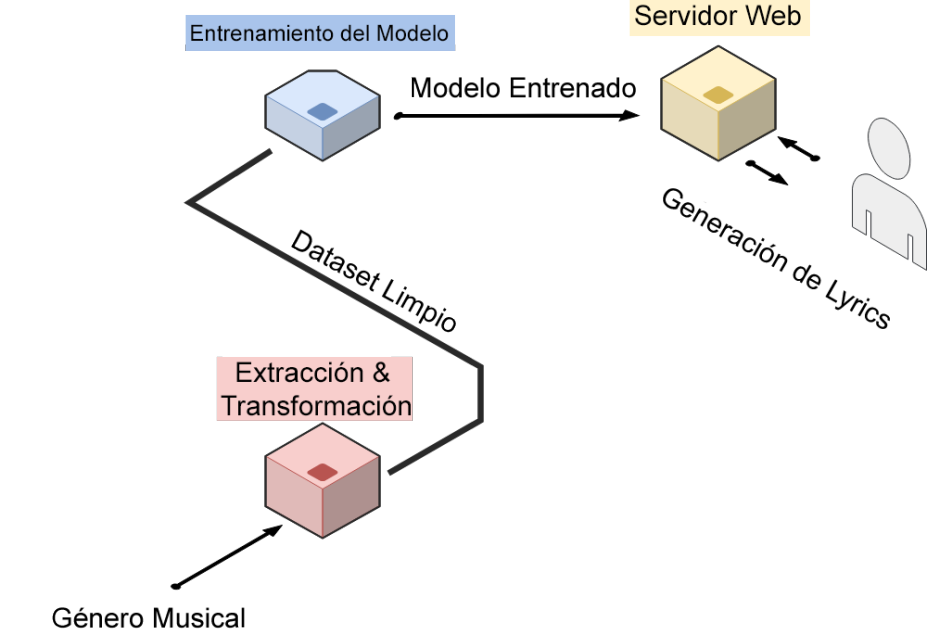
\includegraphics[width=13.5cm]{./Imagenes/Diagramas/general.png}
		\centering \caption{Diagrama general del sistema}
	\end{figure}
	\newpage
	\section{Base de datos}
	El primer paso realizado fue la obtención de una base de datos que contuviera letras de canciones pertenecientes al género musical con el que íbamos a trabajar, que en este caso fue del género pop, y que se encontraran en el idioma inglés. Se hizo una búsqueda de datasets, en distintas plataformas, que cumplieran con los requisitos ya mencionados y que estuvieran disponibles para su uso libre, es decir, que fueran del tipo open source.\\\\
	En la plataforma Kaggle \cite{kaggle} se encontró un dataset titulado “Song lyrics for 6 musical genres” \cite{kaggleDataset} el cual contiene todos los datos necesarios y cumplía con los requisitos buscados para el sistema con un total de 160,790 letras de canciones y cuya información se muestra a continuación como se vería en una base de datos, esto es, en tablas: 
	\begin{figure}[H]
		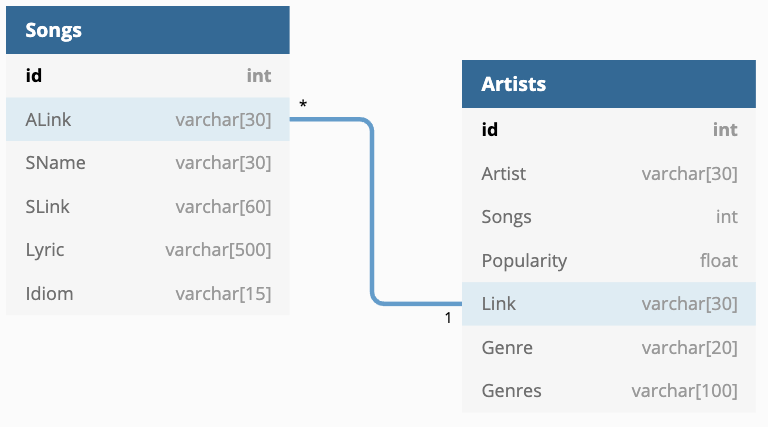
\includegraphics[width=12cm]{./Imagenes/BasedeDatos/diagrama_ER_BD.jpg}
		\centering 
		\caption{Diagrama entidad-relación de la base de datos}
	\end{figure}
	La base de datos de Kaggle se obtuvo originalmente de la página de vagalume.com \cite{vagalume} e incluye 6 tipos de géneros musicales mencionados a continuación.
	\begin{itemize}
		\item Rock
		\item Pop
		\item Hip Hop
		\item Samba
		\item Sertanejo
		\item Funk Carioca
	\end{itemize}
	Como se puede ver, se contaba con la columna “Genre” la cual fue utilizada para separar el dataset en géneros musicales y “Link” la cual se usó como enlace a la segunda tabla. Las tablas fueron fusionadas dando dando como resultado la siguiente:
	\begin{figure}[H]
		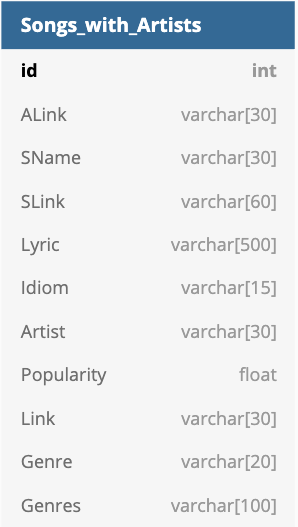
\includegraphics[width=5cm]{./Imagenes/BasedeDatos/Songs_with_Artists.png}
		\centering 
		\caption{Diagrama entidad-relación de la base de datos procesada}
	\end{figure}
	En este punto se requiere extraer la información precisa que se va utilizar para el entrenamiento del modelo, para ello se hace uso de la columna “Lyric” y así seleccionar las letras que se usarán para entrenar el modelo, “Idiom” para separar las canciones en el idioma inglés y la columna de “Genre” para tamizar las canciones que forman parte del género pop, formando así una base de datos simple que contiene únicamente las letras de canciones del género pop en el idioma inglés.
	\begin{figure}[H]
		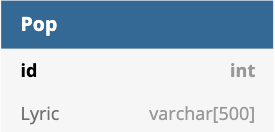
\includegraphics[width=5cm]{./Imagenes/BasedeDatos/Pop.png}
		\centering 
		\caption{Diagrama entidad-relación final}
	\end{figure}
	\newpage
	\section{Limpieza de la base de datos}
	Una vez obtenida la base de datos, es necesario hacer una inspección de esta misma para verificar que los estos datos sean útiles para proceder a generar un modelo, este paso resulta de suma importancia, ya que de esto depende que la precisión de los resultados del modelo.\\\\
	Para ello se identificarán datos que resulten incompletos, incorrectos, inexactos o no pertinentes para luego sustituirlos, modificarlos o en su caso, eliminar estos datos. \\\\\
	Estas inconsistencias en el conjunto de datos pueden ser causados por errores de entrada del usuario, corrupción de los datos, errores al realizar el scraping, o simplemente cuenta con caracteres que no nos interesa procesar. Una vez realizada esta limpieza, la base de datos será conciliable para usarse en el entrenamiento y así los resultados generados finales tendrán una mejor comprensión. \\\\
	Para ello se utilizó la librería de “Pandas” así como la librería de expresiones regulares. Para limpiar los datos se siguió el estándar de limpieza de datos: \cite{data_cleaning}
	\begin{enumerate}
		\item Remover caracteres innecesarios
		\item Eliminar Duplicados
		\item Evitar errores ortográficos de similitud
		\item Convertir los tipos de dato
		\item Tratar los valores nulos o faltantes
	\end{enumerate}
	Con la limpieza del conjunto de datos se tuvo como resultado una base de datos útil solo con los datos necesarios para poder tratarlos con el debido proceso para empezar el entrenamiento del modelo de la red neuronal, este proceso es necesario hacer solo una sola vez para cada género musical ingresado, en caso de que se lleguen a necesitar más datos, será necesario repetir el proceso para poder generar resultados de la manera más óptima posible. A continuación, se muestran las primeras líneas de la base de datos limpias.
	\begin{figure}[H]
		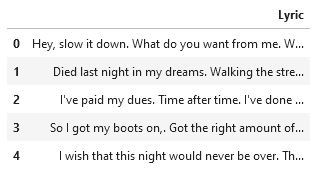
\includegraphics[width=7cm]{./Imagenes/BasedeDatos/ResultadosLimpiezaBasedeDatos.png}
		\centering 
		\caption{Resultados de limpieza en la base de batos}
	\end{figure}
	\newpage
	\section{Desarrollo del modelo}
	Para el desarrollo del modelo se utilizó una libreta de Kaggle. El lenguaje de programación utilizado para el desarrollo del modelo fue Python, y lo primero que se hizo en la libreta de Kaggle fue la importación de las librerías que se fueran a necesitar, siendo las más importantes:	
	\begin{itemize}
		\item Pandas: permite manipular y analizar la información.
		\item Tensorflow: herramienta que ayuda en el procesamiento del aprendizaje automático.
		\item Keras: herramienta que ayuda en el procesamiento del aprendizaje profundo.
	\end{itemize}
	Llegados a este punto se procede a importar el conjunto de datos previamente limpiado, apoyándonos ahora de la librería de Pandas y conservando únicamente la letra de las canciones, ya que es la información con la que nos interesa trabajar y la cual vamos a estar manipulando.\\\\
	Al usar Kaggle debemos tomar en consideración sus limitantes, siendo algunas de ellas el solamente contar con 16Gb de RAM, un disco de 73Gb y una GPU de 13GB para el procesamiento de nuestro conjunto de datos, razón por la cual debemos limitar nuestro modelo y así en lugar de utilizar todos los datos (28,441), por el momento sólo podemos trabajar de manera estable con 700 letras de canciones.\\\\
	Haciendo uso de esas 700 letras se decidió obtener información específica, como el número de palabras en cada canción con el fin de determinar la frecuencia de distribución del número de palabras de cada texto, y así tener una idea del promedio de palabras al momento de realizar la generación de texto.
	\begin{figure}[H]
		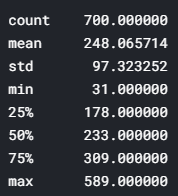
\includegraphics[width=5cm]{./Imagenes/Modelo/estadistica.png}
		\centering 
		\caption{Estadísticas de las palabras}
	\end{figure}
	Lo que podemos observar en la imagen anterior es:
	\begin{itemize}
		\item Count: el número de canciones analizadas.
		\item Mean: el promedio de palabras por canción.
		\item Std: la desviación estándar de las palabras.
		\item Min: la menor cantidad de palabras encontradas en una canción.
		\item Max: la mayor cantidad de palabras encontradas en una canción.
	\end{itemize}
	Aunado a esto, se le realizó una tokenización a las letras de nuestras 700 canciones, esto significa que se separo cada palabra, y cada una se convirtió en un número. Este proceso se llevo acabo con el uso de Keras y la clase Tokenizer(), la cual cuenta con dos métodos importantes:
	\begin{itemize}
		\item \_fit\_ontext(): Actualiza el vocabulario interno en función de una lista de textos determinada o, en este caso, la columna “Lyrics”, donde cada entrada de la lista será un token.
		\item \_texts\_tosequences(): Transforma cada texto dentro de la lista de textos proporcionados en una secuencia de números enteros; solo se considerarán las palabras conocidas por el tokenizador.
	\end{itemize}	
	\begin{figure}[H]
		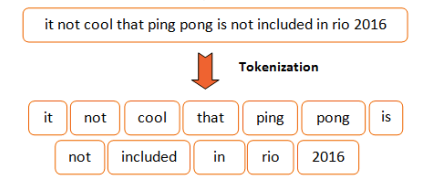
\includegraphics[width=10cm]{./Imagenes/Modelo/tokenization.png}
		\centering 
		\caption{Tokenizado de las palabras \cite{tokenimagen}}
	\end{figure}
	Antes de la generación del modelo es necesario normalizar todas las oraciones a una misma longitud estándar para evitar el desbordamiento de la memoria y conseguir así que las capas del modelo sean mucho más profundas, este es un proceso simple conocido como “Padding”, el cual agrega ceros al comienzo del texto dando como resultado capas del mismo tamaño.\\\\
	La posición donde se agregarán los ceros viene determinada por el “Padding”, en este caso, se hará al comienzo de la secuencia.
	\begin{figure}[H]
		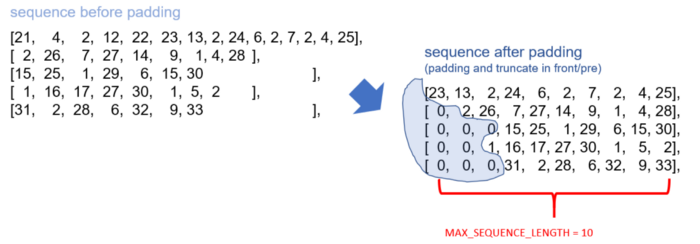
\includegraphics[width=10cm]{./Imagenes/Modelo/padding.png}
		\centering 
		\caption{Padding del tokenizado de las palabras}
	\end{figure}	
	\newpage	
	\section{Creación del modelo}
	Se utilizó un modelo del tipo LSTM Bidireccional, este tipo de redes neuronales se ejecutan como su nombre lo indica: en dos direcciones. Esto quiere decir que va del pasado al futuro y viceversa, así es como el modelo conserva la información de ambos estados en cualquier momento. Las redes neuronales del tipo LSTM se utilizan principalmente cuando el contexto importa.\\\\
	Los modelos en Keras se definen como una secuencia de capas, y las capas son el componente básico de la red neuronal. Algunos ejemplos de tales capas son:
	\subsection{Embedding o incrustación}
	Es una capa central, solo es posible usarla como la primera capa en un modelo, convierte los números enteros positivos en vectores densos de un tamaño fijo (el primer parámetro es el tamaño del vocabulario, el segundo parámetro es la dimensión de la incrustación densa, y el tercer parámetro trata la longitud de las secuencias, este se requiere ya que se hará uso de una capa del tipo Denso más adelante).
	\begin{center}
		\lstinputlisting[language=Python]{./Imagenes/Modelo/embedding.py}
	\end{center}
	\subsection{Bidireccional}
	Es una capa recurrente, una envoltura bidireccional para las redes neuronales de tipo RNN's que recibirá una capa como entrada, siendo la capa LSTM la que elegimos, recibirá un entero positivo como entrada que se refiere a la cantidad de nodos de salida que se deben devolver.
	\begin{center}
		\lstinputlisting[language=Python]{./Imagenes/Modelo/bidireccional.py}
	\end{center}
	\subsection{Dropout}
	Es una capa de regularización. Esta capa establece aleatoriamente las unidades de entrada en 0, con una frecuencia del valor que le pasamos, en cada paso durante el tiempo de entrenamiento, lo que ayuda a evitar el sobre ajuste.
	\begin{center}
		\lstinputlisting[language=Python]{./Imagenes/Modelo/dropout.py}
	\end{center}
	\subsection{Densidad}
	Es una capa central y una capa de red neuronal densamente conectada. Recibe como primer parámetro un entero positivo que se refiere a la cantidad de nodos de salida que deben devolverse. El segundo parámetro es el llamado activación que define el tipo de predicciones que puede hacer el modelo; para el tipo de problema que estamos considerando, el que se adapta mejor es softmax, que genera un vector de valores (entrada) que puede interpretarse como probabilidades de ser utilizado.
	\begin{center}
		\lstinputlisting[language=Python]{./Imagenes/Modelo/dense.py}
	\end{center}
	\subsection{Método de compilación, algoritmo de optimización y métrica de rendimiento}
	“Loss”: También conocida como función de costos; funciona durante el proceso de optimización y su trabajo es calcular el error del modelo. La entropía cruzada se utiliza para estimar la diferencia entre una distribución de probabilidad estimada y predicha. Se utilizará categorical\_cross-entropy porque es más adecuado para este tipo de problemas y se usa casi universalmente para entrenar redes neuronales de aprendizaje profundo debido a los resultados que produce.\\
	“Optimizer”: Su tarea es reducir las pérdidas y brindar los resultados más precisos posibles. Adam es la opción elegida debido a que es la mejor opción que ofrece Keras para entrenar la red neuronal en el menor tiempo y de la forma más eficiente.\\
	“Earlystop”: Detendrá el entrenamiento si el modelo ha dejado de mejorar, y esto es comprobado al final de cada “epoch” o iteración.\\
	En este caso, la “precisión” o “accuracy” se utilizará como métrica de rendimiento.
	“fit”: Encargado de entrenar el modelo por un número fijo de epochs dados.	
	\begin{center}
		\lstinputlisting[language=Python]{./Imagenes/Modelo/compile.py}
	\end{center}
	El código del modelo queda entonces de la siguiente forma:
	\begin{center}
		\lstinputlisting[language=Python]{./Imagenes/Modelo/modelo.py}
	\end{center}
	\subsection{Importación del modelo}
	Una vez completado el entrenamiento de nuestro modelo, sólo queda importarlo y así probar su funcionamiento, en nuestro caso nombramos al modelo “song\_lyrics\_generator” y se importó de la siguiente manera, llamando al enlace de nuestra libreta de Kaggle:
	\begin{center}
		\lstinputlisting[language=Python]{./Imagenes/Modelo/import.py}
	\end{center}
	Una vez que contamos con el modelo importado se crea una función que se usará para generar la letra de una canción utilizando el modelo previamente entrenado, y éste predecirá las siguientes palabras tomando como contexto a la(s) palabra(s) de entrada suministradas como “seed\_text”. Para que esto funcione, se debe aplicar una tokenización al seed\_text, posterior a ello se aplicará un padding a las secuencias generadas y se pasarán al modelo entrenado, obteniendo de esta manera que se pueda predecir la siguiente palabra.
	\begin{center}
		\lstinputlisting[language=Python]{./Imagenes/Modelo/function.py}
	\end{center}	
	\newpage
	\section{Desarrollo de la aplicación web}
	El desarrollo de la aplicación web fue llevado a cabo haciendo uso de React, mejor conocida como ReactJS, la cual es una biblioteca de Javacript usada en mayor parte para la creación de interfaces interactivas diseñadas sobre componentes, los cuales una vez renderizados son mostrados al usuario final.\\\\
	La biblioteca fue escogida debido a que hace posible la compatibilidad con dispositivos móviles sin la necesidad de escribir código específico para esta tecnología, esto es, nos ofrece un estado responsivo que cambie en función del dispositivo donde se muestre la aplicación web.\\\\
	Previo a empezar el trabajo con React fue necesario descargar “Node.js” desde su página (https://nodejs.org/es/) el cual permite crear aplicaciones web utilizando Javascript, y al haberlo instalado se obtiene el comando “npm” usado en la terminal, el cual permite instalar paquetes al proyecto sobre el que se trabaje posibilitando la adición de nuevas funciones a nuestra aplicación web.\\\\
	Teniendo instalado Node.js y haciendo uso de una terminal es necesario escribir el comando “npm start”, el cual ejecuta un servidor de desarrollo de forma local al que se puede acceder colocando la dirección “localhost:3000” en cualquier navegador, donde se mostrará cómo va quedando el proyecto sobre el que se esté trabajando.\\\\
	Para el diseño de la aplicación web nos enfocamos en que su estructura se trabajara bajo el entendido de que las pestañas que se fueran a mostrar sean aquellas que consideramos como las más relevantes, siendo estas: Página de Inicio, Preguntas Frecuentes, Ejemplos de letras de canciones previamente generadas y una acerca del equipo.\\\\
	\begin{figure}[H]
		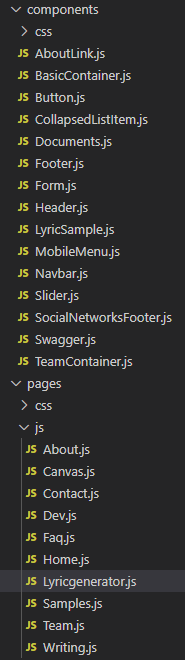
\includegraphics[width=5cm]{./Imagenes/AplicacionWeb/Paginas.png}
		\centering 
		\caption{Páginas trabajadas}
	\end{figure}
	Entre todo el diseño, la página principal es la más importante debido a que esta es la primera que ve el usuario al acceder a la aplicación web y con la que más va a interactuar durante su estadía; lo primero que se muestra es un mensaje con un botón verde, colocado con clara intención de invitar al usuario a presionarlo.
	\begin{figure}[H]
		\includegraphics[width=13.5cm]{./Imagenes/AplicacionWeb/Paginaweb.png}
		\centering 
		\caption{Página de bienvenida}
	\end{figure}
	Si el usuario decide presionar el botón será llevado a un formulario sin necesidad de pasar a otra página, maximizando así la sensación de no demora, donde inmediatamente se le es requerido que introduzca una palabra en el idioma inglés en el único campo de entrada de texto, teniendo así la posibilidad de regresar al inicio o de generar la letra con la palabra proporcionada.
	\begin{figure}[H]
		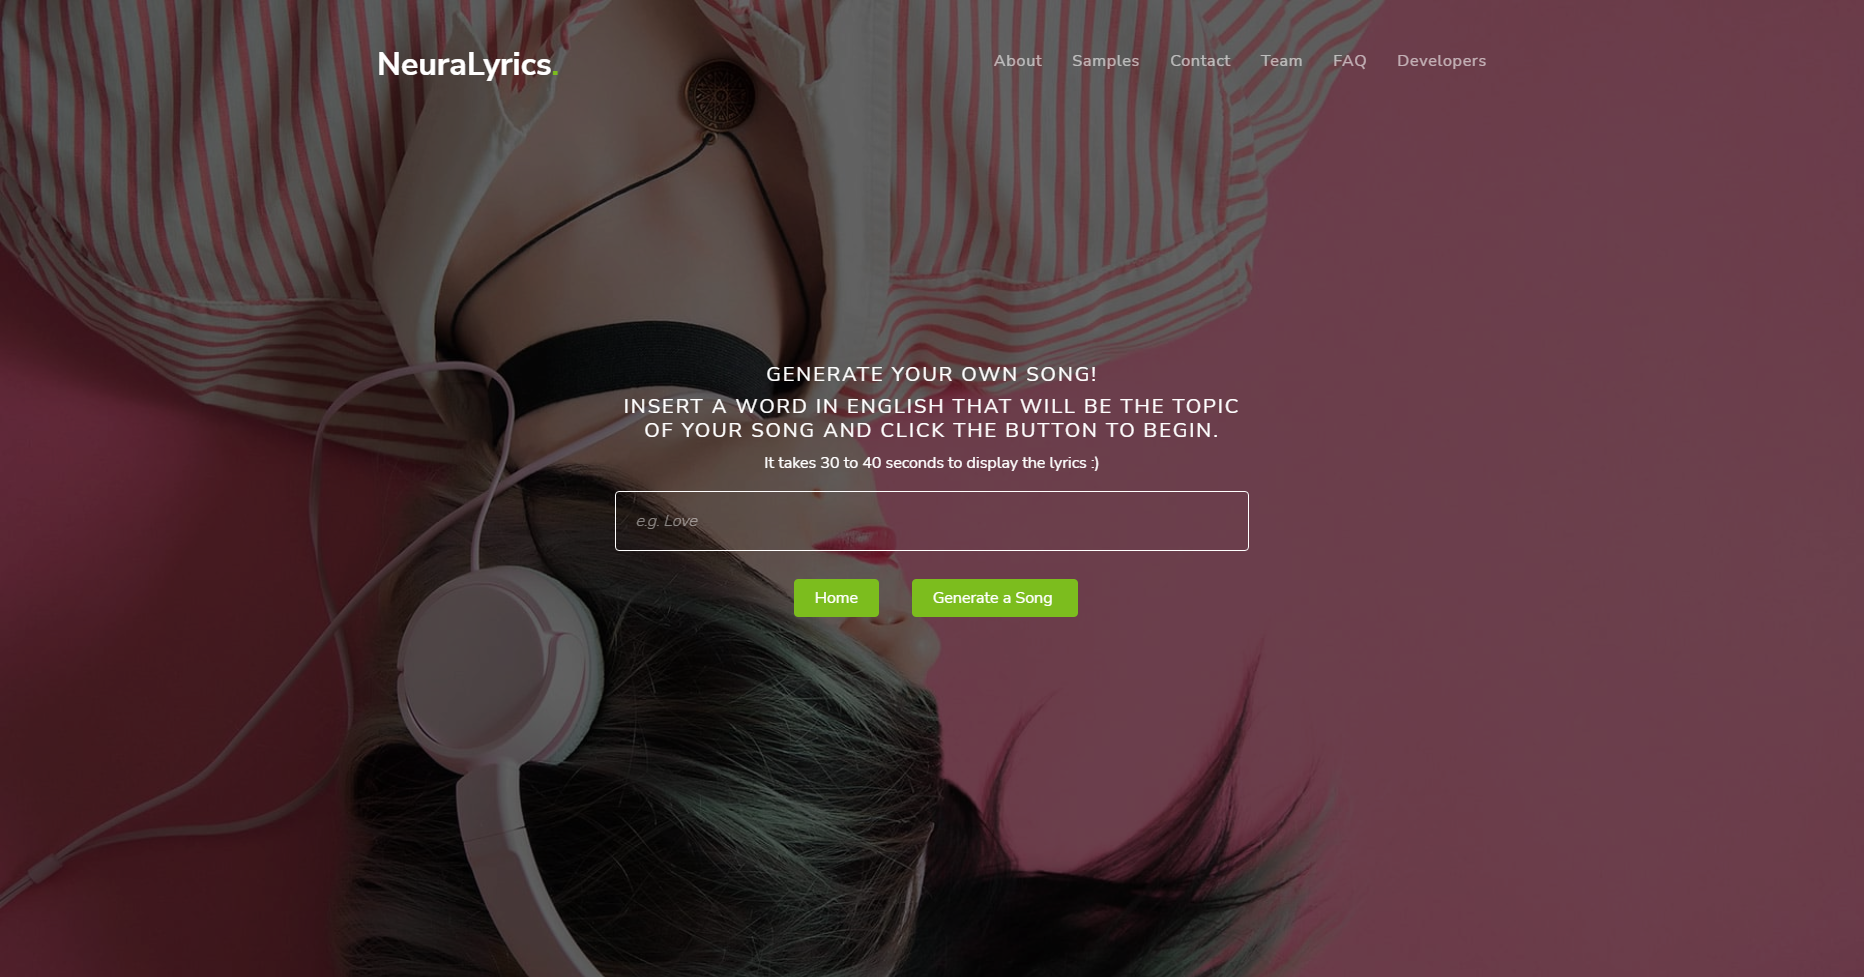
\includegraphics[width=13.5cm]{./Imagenes/AplicacionWeb/pform.png}
		\centering 
		\caption{Formulario}
	\end{figure}
	Se hace una pausa para mostrar la manera en que el dato proporcionado por el usuario es leído y enviado al servidor para ser procesado por el modelo, y así un resultado más personalizados pueda ser devuelto. A continuación, se presenta el código utilizado para la realización de este proceso.
	\begin{center}
		\lstinputlisting[language=JavaScript]{./Imagenes/AplicacionWeb/Sendword.js}
	\end{center}
	Lo que recibe la función es la palabra que introdujo el usuario, esto es hecho ubicando el identificador del campo de texto y obteniendo su valor, el cual es enviado al servidor mediante el uso de la función “fetch”, lo que hace dicha función es buscar la url que se le proporciona (donde se encuentra alojado el servidor) y busca el método post el cual espera recibir los datos en formato Json; los datos proporcionados por el usuario deben ser enviados al servidor en formato json.\\\\
	Si el usuario decide presionar el botón de Generar Canción será desplegada una leyenda que pide aguardar unos segundos en lo que queda generada la letra. Segundos después, la letra de la canción generada irá siendo actualizada y mostrada al usuario dando un efecto de ser escrita al momento; aparecerán al final de la letra 3 botones, el primero permite descargar la letra generada en un archivo de texto, el segundo posibilita al usuario el generar una nueva canción utilizando la misma palabra con la que genero la letra actual pero esperando un resultado distinto, y el último botón regresa a la interfaz previa si lo que se busca es generar una nueva letra con una palabra distinta a la ya usada.
	\begin{figure}[H]
		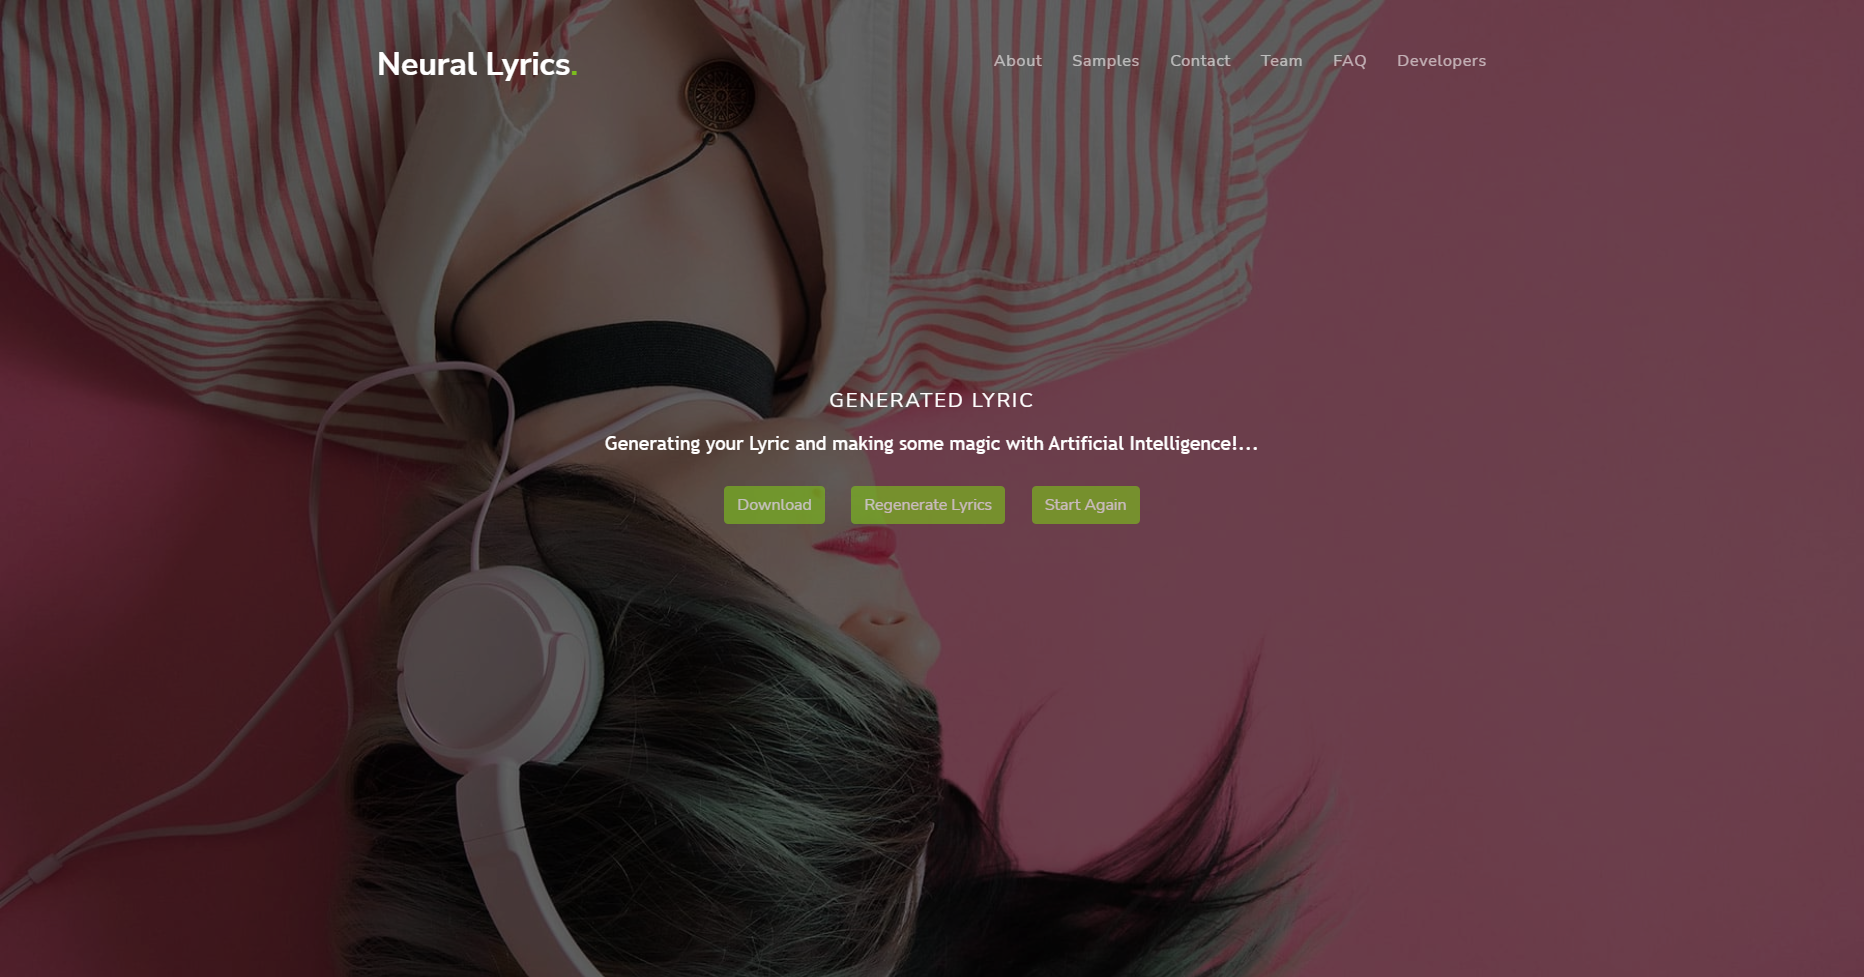
\includegraphics[width=13.5cm]{./Imagenes/AplicacionWeb/pgenerating.png}
		\centering 
		\caption{Leyenda mostrada}
	\end{figure}
	\begin{figure}[H]
		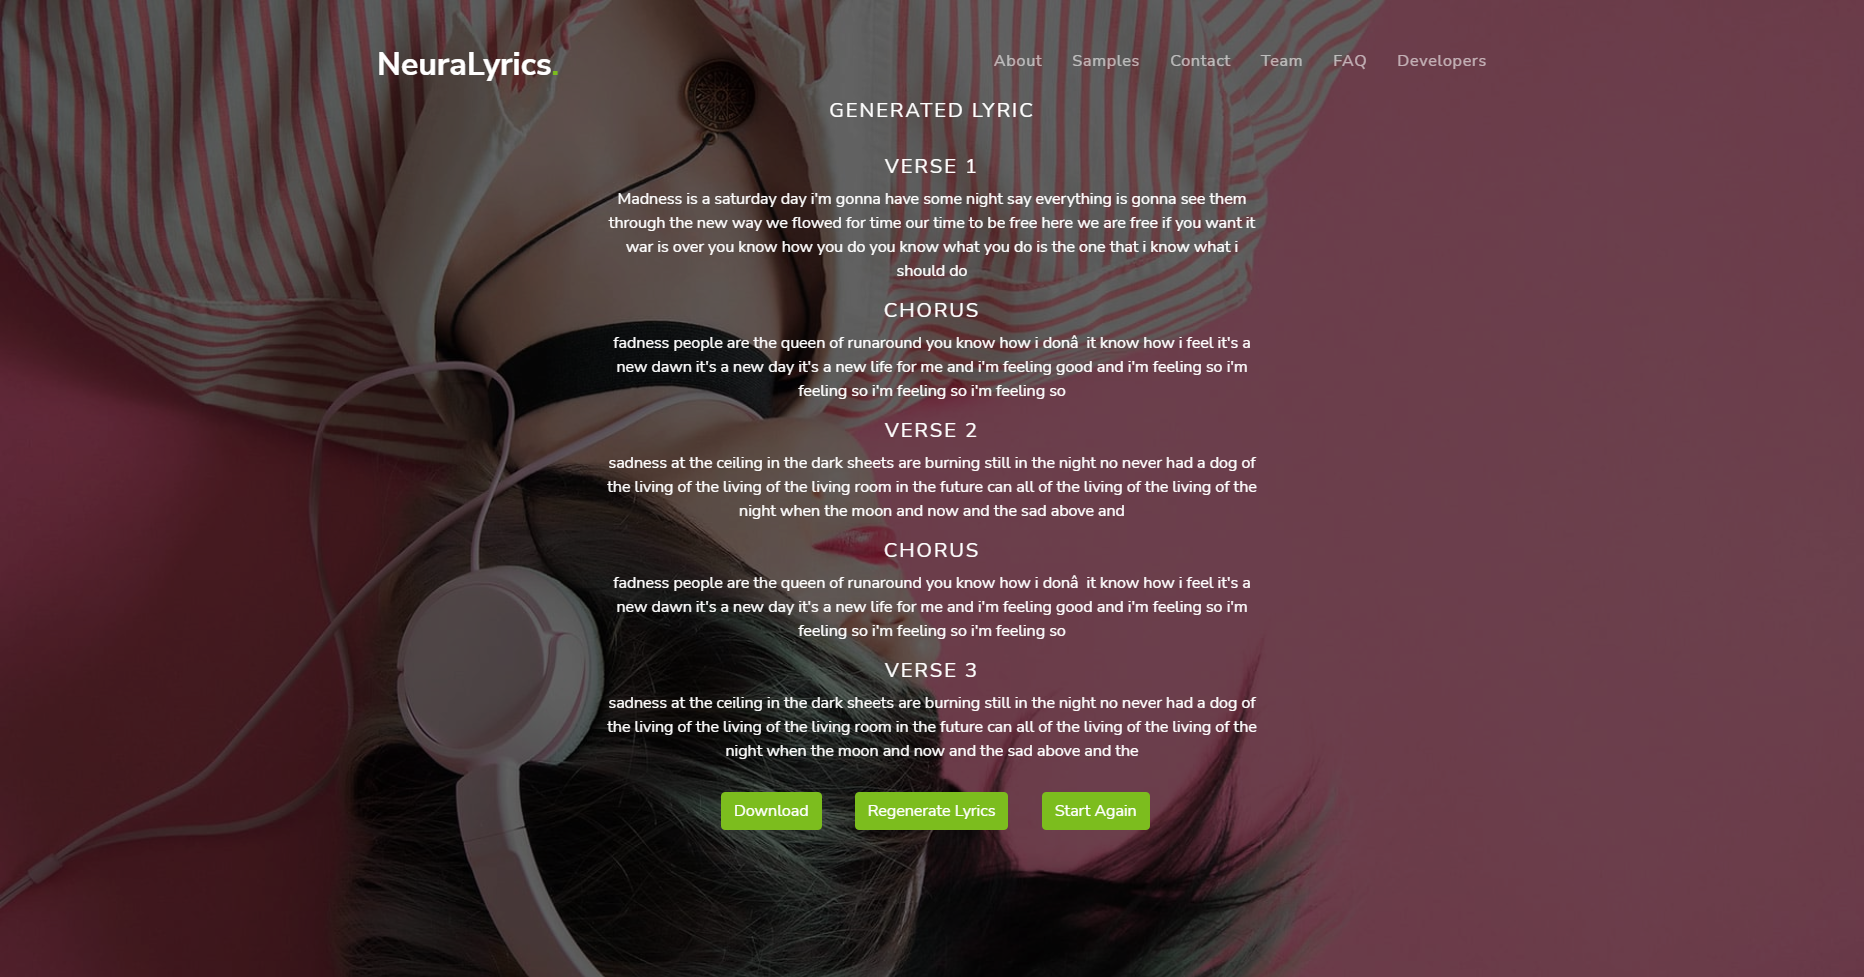
\includegraphics[width=13.5cm]{./Imagenes/AplicacionWeb/Generated.png}
		\centering 
		\caption{Texto generado}
	\end{figure}
	\newpage
	\begin{center}
		\lstinputlisting[language=JavaScript]{./Imagenes/AplicacionWeb/ModelConection.js}
	\end{center}
	El código anterior tiene como objetivo el actualizar la pantalla con una serie de textos pensados para la espera, de manera tal que el usuario vea que se sigue trabajando y no piense que el sitio se congeló, una vez que la letra es recibida se detendrá la generación de datos curiosos y se desplegarán los versos y coros.
	\begin{center}
		\lstinputlisting[language=JavaScript]{./Imagenes/AplicacionWeb/Download.js}
	\end{center}
	La función “download” permite crear un archivo de texto conteniendo la letra de la canción que se generó en ese momento y descargarla al dispositivo que se esté usando.
	\begin{figure}[H]
		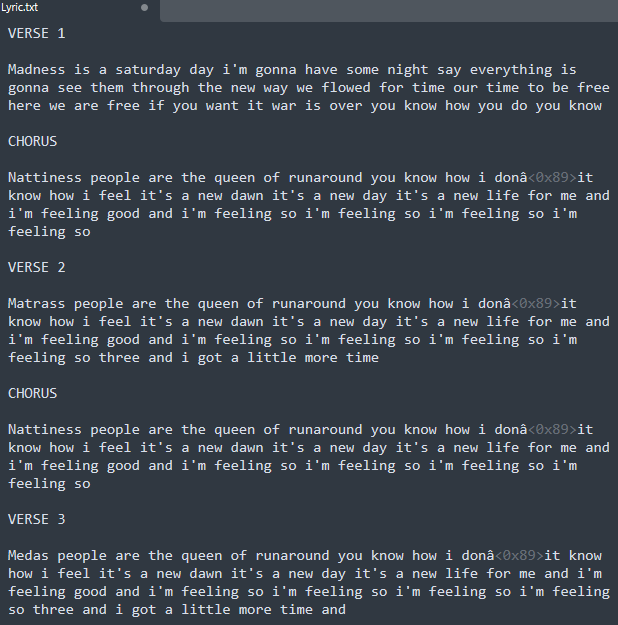
\includegraphics[width=10cm]{./Imagenes/AplicacionWeb/Archivo.png}
		\centering 
		\caption{Archivo de texto descargado}
	\end{figure}	
	El segundo botón hace uso de la misma función y el mismo parámetro con los que se genera la letra, esto es, se reenvía al backend los parámetros utilizados y los elementos dentro de la ventana son renderizados nuevamente mostrando una vez la serie de datos curiosos en lo que se recibe respuesta del servidor.\\
	El tercer botón tiene como función regresar al usuario al campo de texto donde puede ingresar la palabra con la que quiere que se genere la letra de la canción.
	\newpage
	\section{Desarrollo del backend}
	Se tomó la decisión de trabajarlo con una aplicación web desarrollada en Flask, esto debido a que la implementación es relativamente fácil y rápida de lograr aunado a que permite una mejor integración con el modelo y la aplicación web trabajada en React.\\\\
	Para poder trabajar con una aplicación web en Flask lo primero que se requiere hacer, o que se recomienda, es crear un ambiente virtual usando “virtualenv” con la finalidad de separar las librerías Python instaladas originalmente en la computadora de las que se requieren por el proyecto con el que se va a trabajar. Una vez se tiene esto preparado, se procede al desarrollo del código.
	\begin{center}
		\lstinputlisting[language=Python]{./Imagenes/BackEnd/app.py}
	\end{center}
	El código anterior se puede encontrar en el archivo “app.py”, es el código principal de nuestro backend y se despliega en el navegador web; muestra información relacionada a la aplicación que se está trabajando como su nombre, versión y los plugins con los que esta cuenta.\\\\
	Con el objetivo de dar mayor claridad a la manera en que funciona el backend, se realizó una pequeña interfaz a la que es posible acceder desde la siguiente dirección “https://www.neuralyrics.com/developers” y en ella podemos encontrar desglosado en mayor detalle el status actual de la API, la cual se encuentra ubicada en el espacio que lleva por nombre “Health”.
	\begin{figure}[H]
		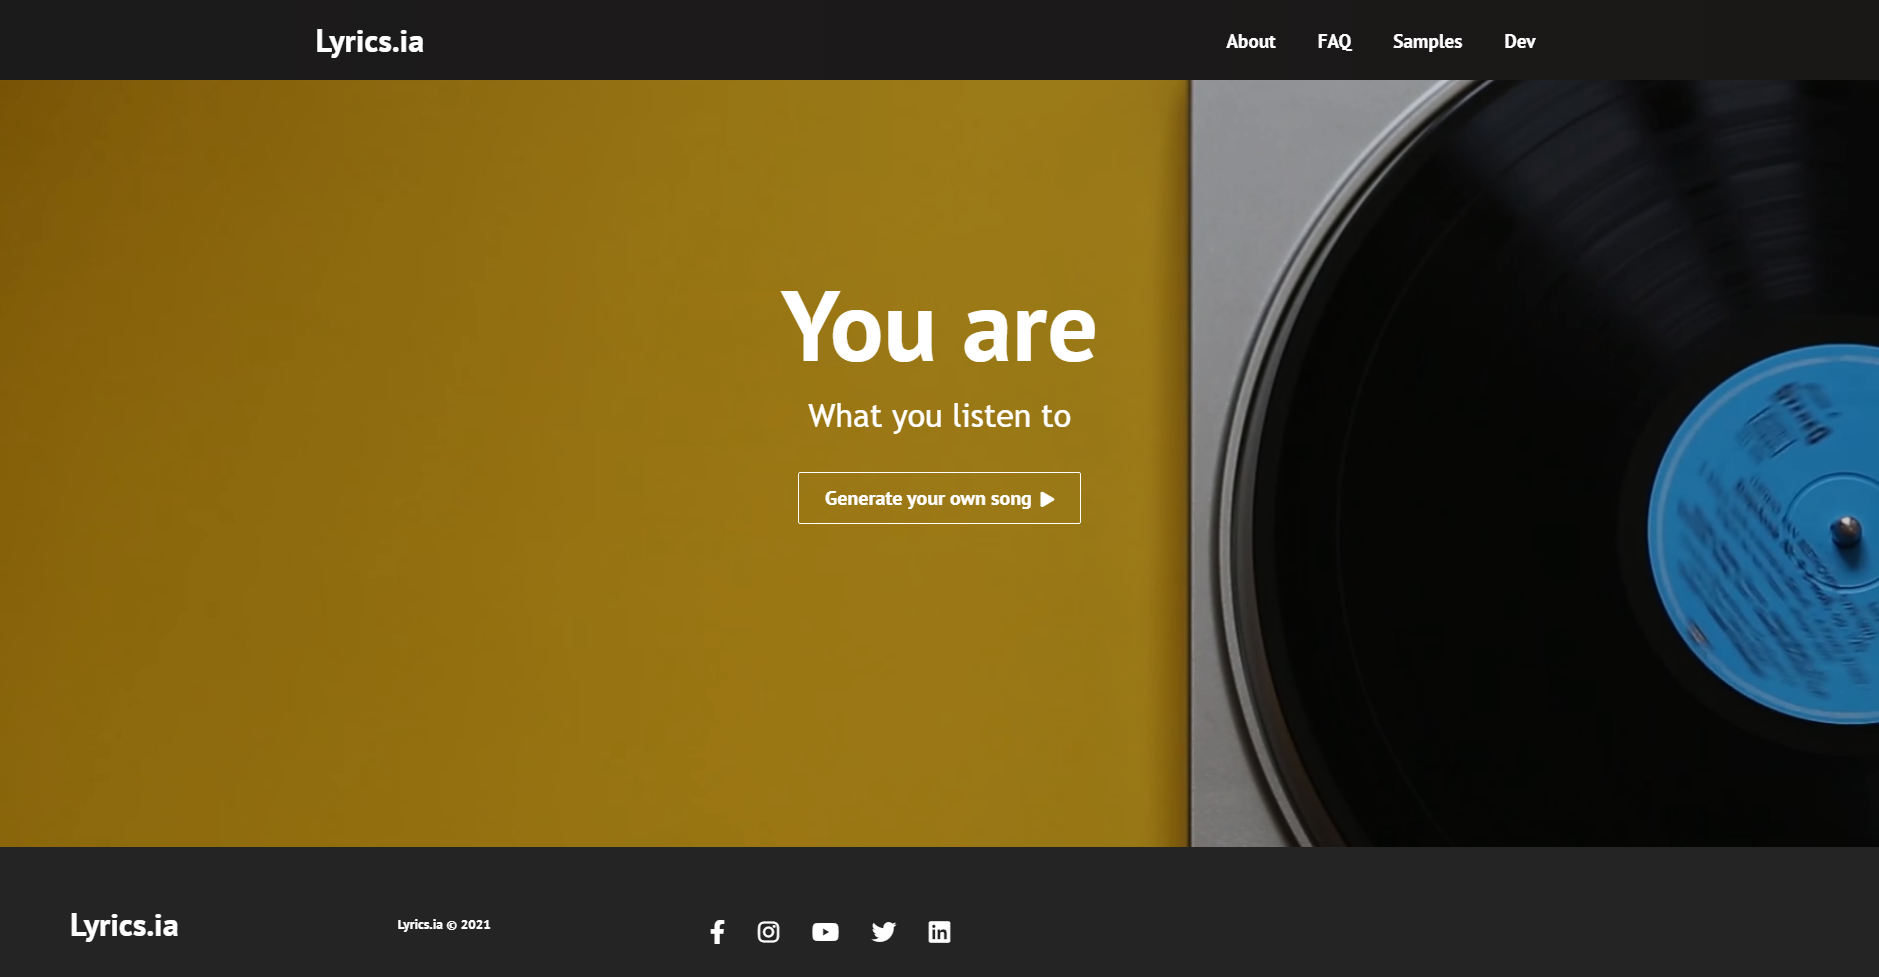
\includegraphics[width=13.5cm]{./Imagenes/BackEnd/Health.png}
		\centering 
		\caption{Cuadro de status del Backend}
	\end{figure}
	Yéndonos más abajo dentro de la misma dirección se puede encontrar el método post de la API, el cuál tiene como tarea el recibir la información de la aplicación web realizada en React en formato json, y así enviar esta información al modelo.
	\begin{figure}[H]
		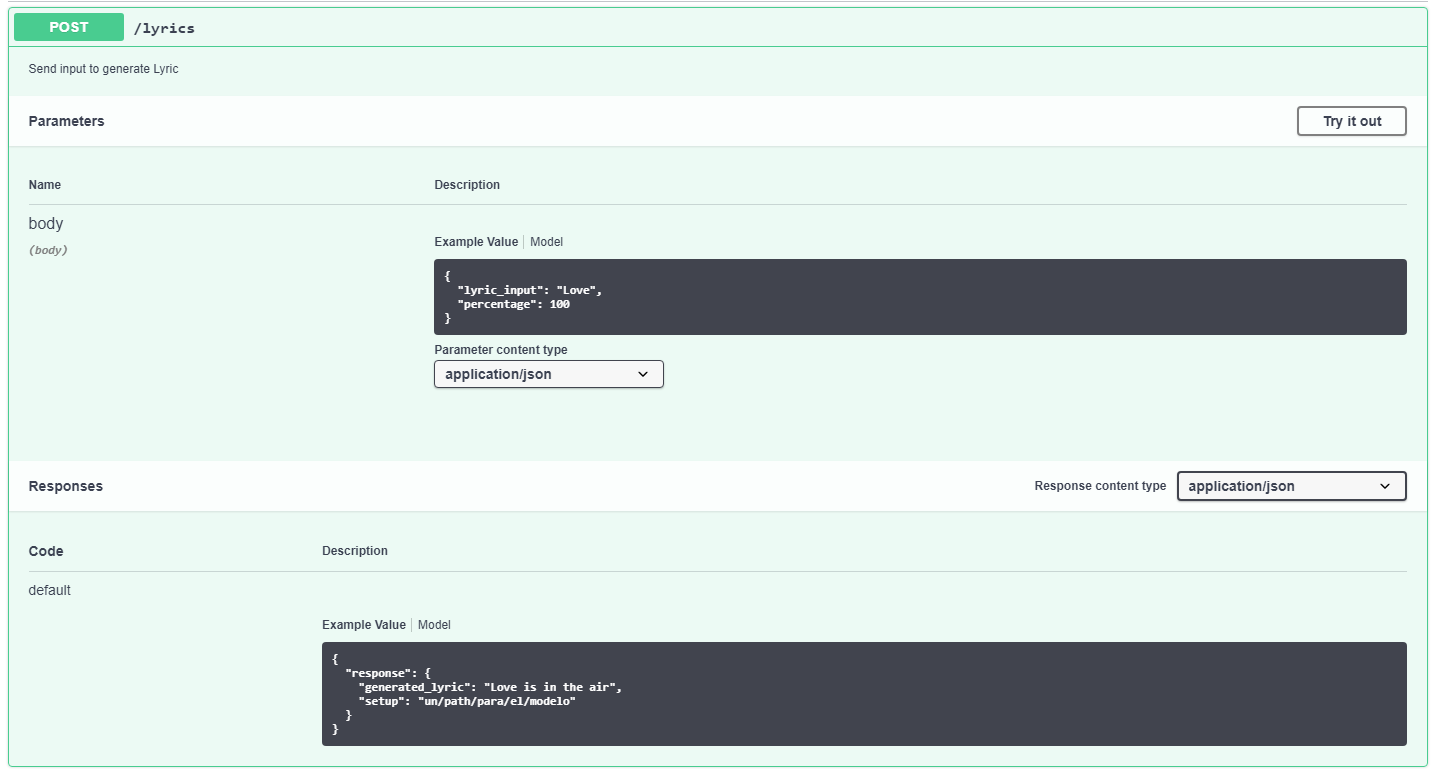
\includegraphics[width=13.5cm]{./Imagenes/BackEnd/Post.png}
		\centering 
		\caption{Cuadro del método Post}
	\end{figure}
	Para realizar esta tarea se desarrolló el siguiente código:
	\begin{center}
		\lstinputlisting[language=Python]{./Imagenes/BackEnd/generate_lyrics.py}
	\end{center}
	La palabra introducida por el usuario es enviada al modelo para ser procesada,  generando de esta manera un texto con la letra de la canción, este procedimiento se realiza en la función “generate\_lyric” y el texto generado es regresado en formato json a la aplicación web en React, que será posteriormente mostrada en el navegador web del usuario.
	\newpage
	\section{Desplegando componentes}
		Una vez se tiene lista la comunicación con el modelo, se vuelve necesario conectar la función para que pueda recibir llamadas por medio de peticiones web, por lo que se desarrolló una API utilizando Flask para recibir dichas peticiones que en local funcionan llamando al “localhost”, y una vez que se establece la comunicación entre la página y la API de forma local se procede a desplegar estos componentes por separado ya que se manejan distintos lenguajes de programación y puede ocasionar error tener todo junto, así como por cuestiones de escalamiento y para evitar errores ocasionadas por las estructuras monolíticas.
		
	\subsection{Despliegue del backend}
		Para poder desplegar la API primero se procede a crear una imagen de Docker donde se corren todos los comandos y se instalan las dependencias necesarias para poder crear un contenedor que incluirá a la API y que pueda correr en cualquier sistema operativo compatible con Docker.
		\begin{figure}[H]
			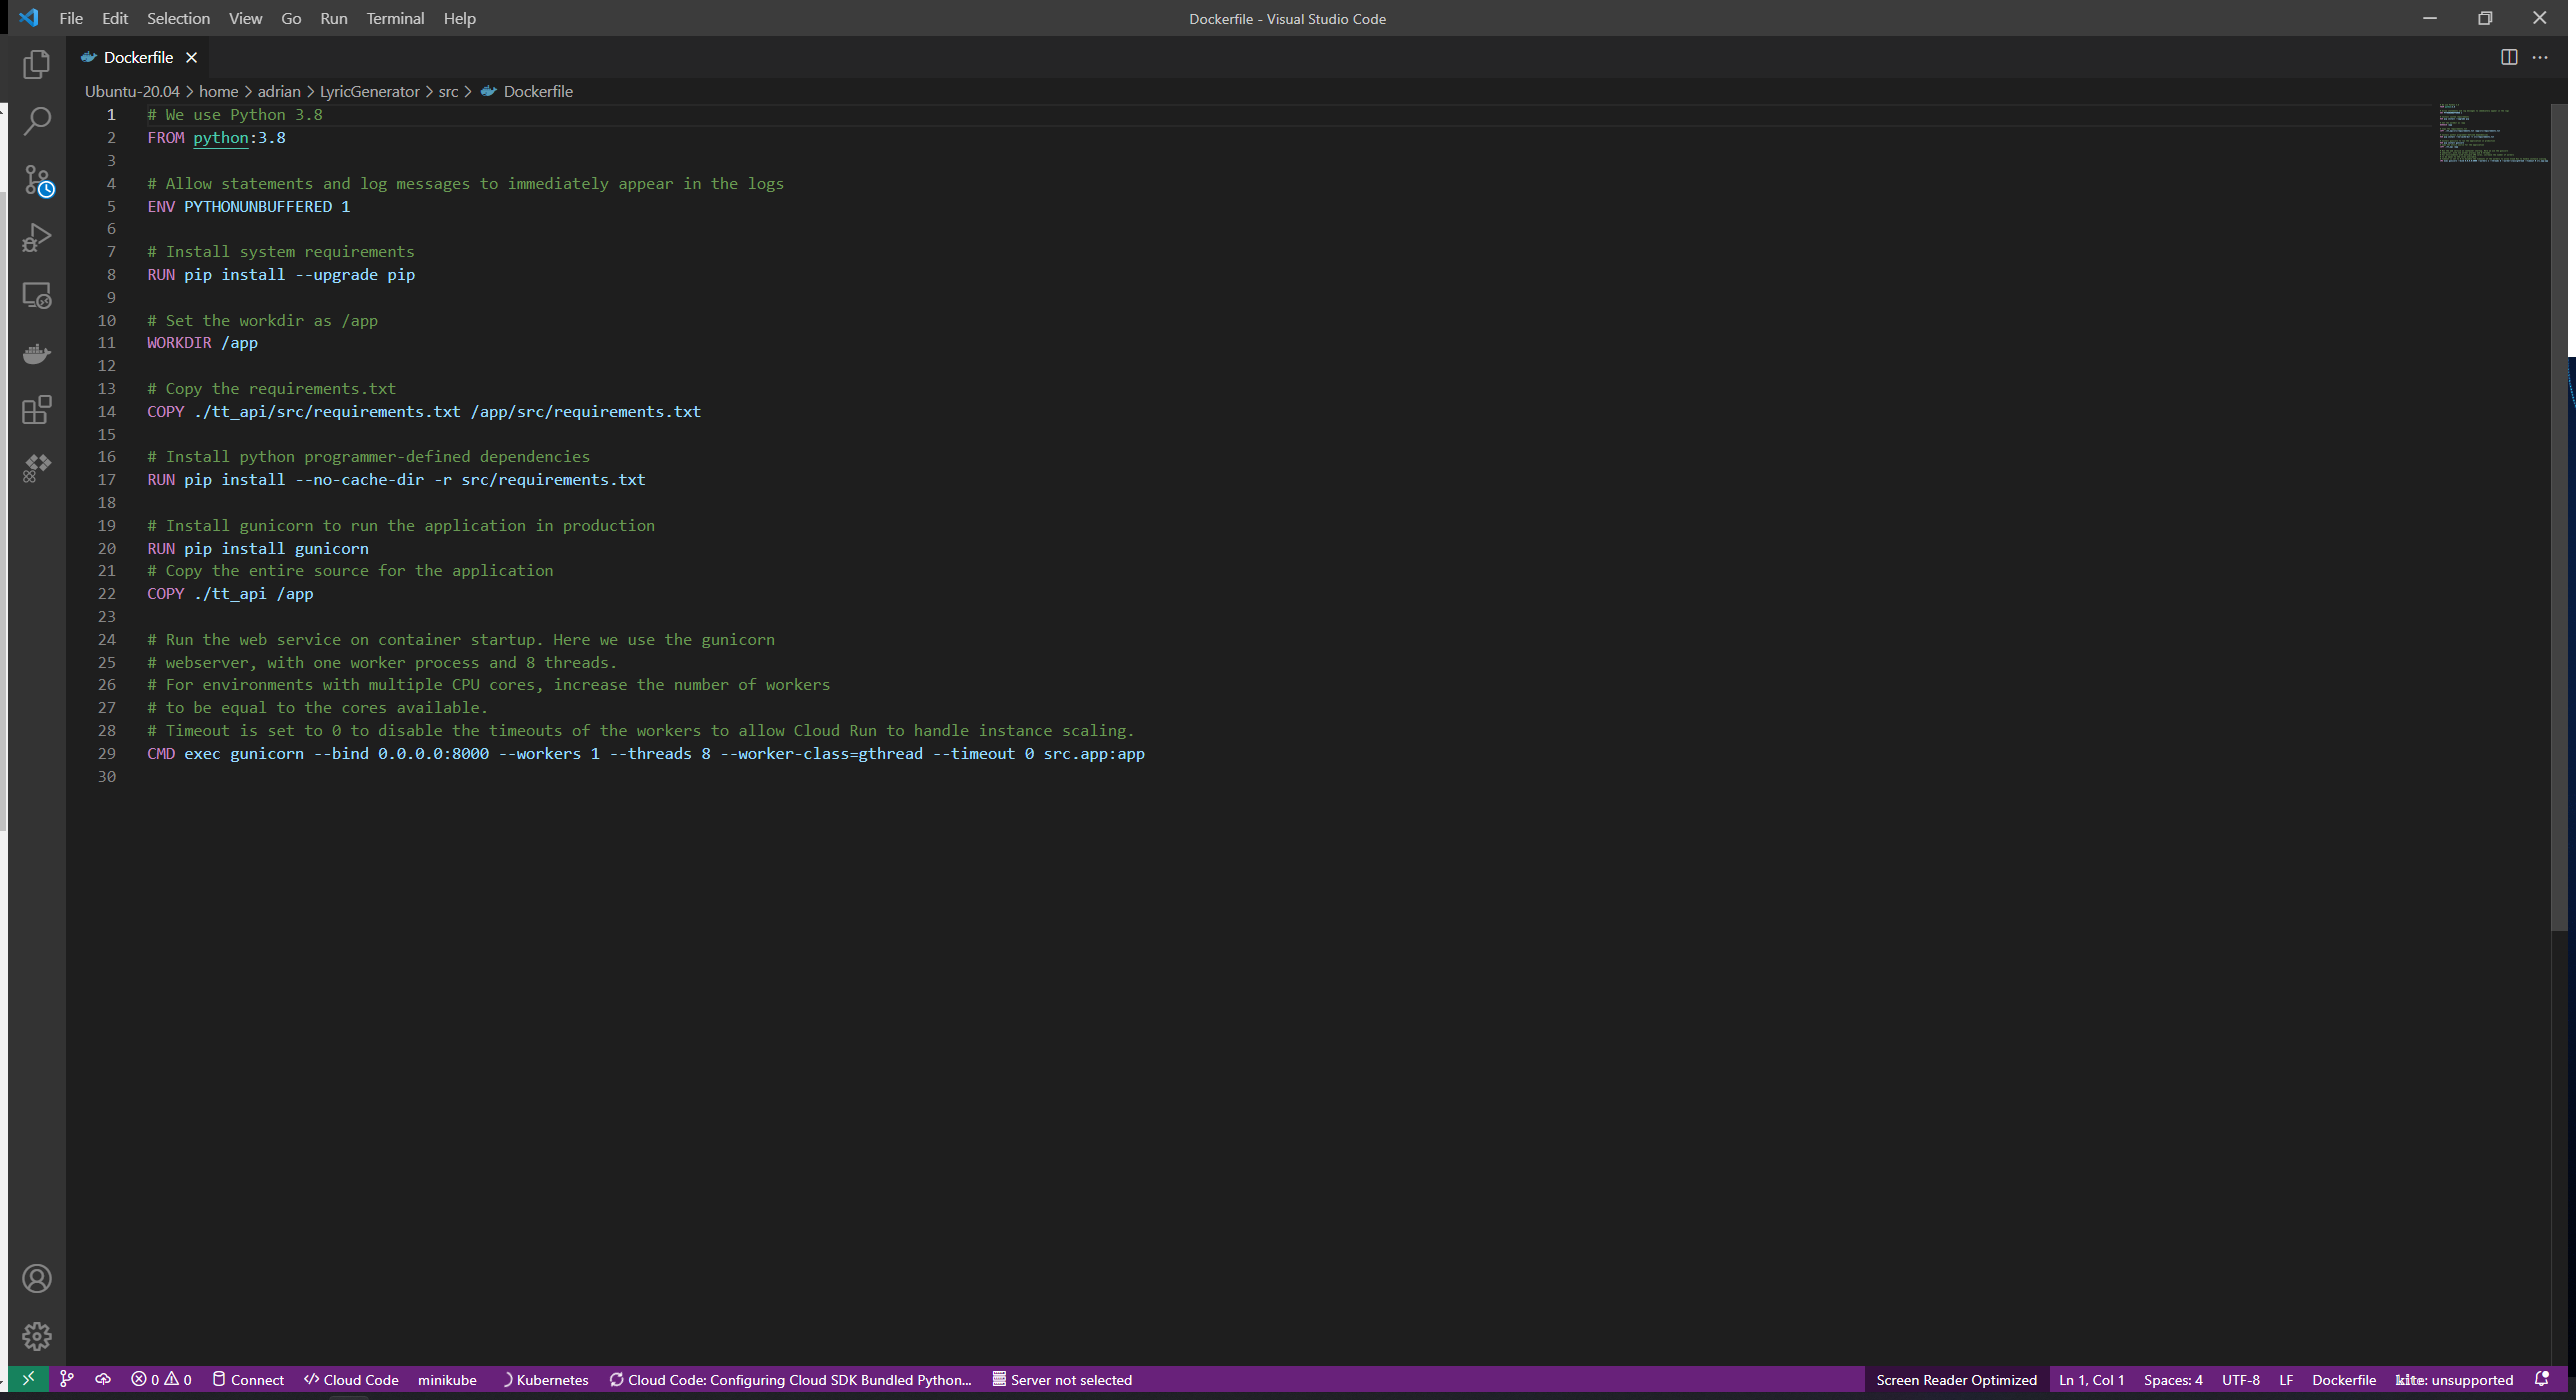
\includegraphics[width=12cm]{./Imagenes/BackEnd/dockerfile.png}
			\centering 
			\caption{Código para la creación de una imagen de Docker con las dependencias necesarias para crear un contenedor con la API.}
		\end{figure}
		Una vez listo el contenedor corriendo localmente, se crea un repositorio con la imagen en un archivo Dockerfile en la plataforma https://hub.docker.com/ con la finalidad de que la herramienta de AWS “Elastic Beanstalk” descargue la imagen desde ahí con una instrucción de un archivo de Docker Compose como se muestra a continuación.
		\begin{figure}[H]
			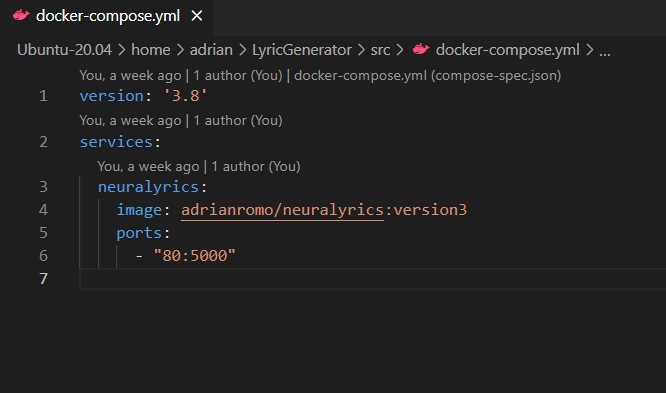
\includegraphics[width=12cm]{./Imagenes/BackEnd/dockercompose.png}
			\centering 
			\caption{Archivo YML con instrucciones para AWS Elastic Beanstalk para subir la imagen correspondiente con la API.}
		\end{figure}
		Una vez se cuenta con los dos archivos, se procede a crear una cuenta en AWS (se recomienda crear un usuario administrador para que se pueda tener acceso a todas las aplicaciones y así configurar las herramientas a conveniencia y según sus necesidades particulares), los pasos a seguir para poder crear un entorno en Elastic Beanstalk son los siguientes:
	
		Se selecciona el tipo de entorno en el que se trabajará, en este caso es un entorno web ya que se trata de una API.
		\begin{figure}[H]
			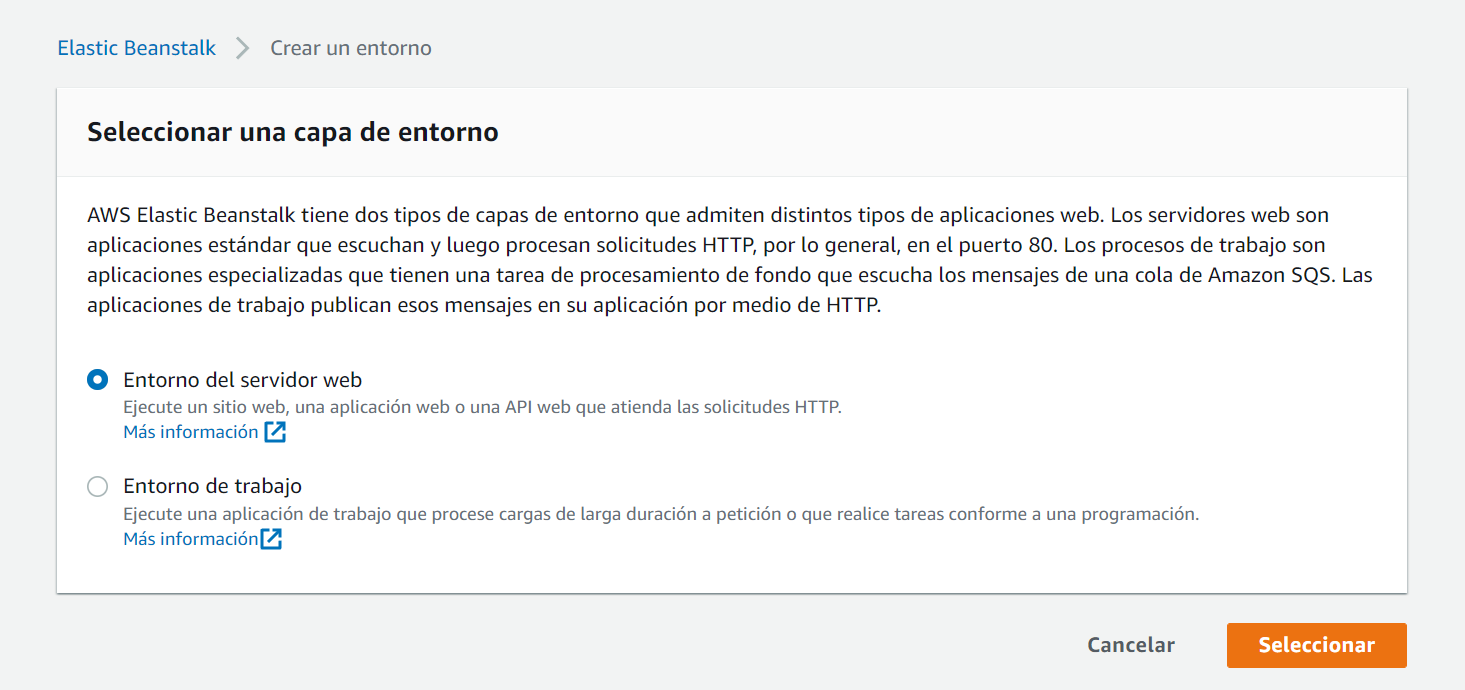
\includegraphics[width=12cm]{./Imagenes/BackEnd/paso_1.png}
			\centering 
			\caption{Tipos de entornos.}
		\end{figure}
		Se le da un nombre al entorno, se elige un nombre para generar el enlace a la API y una breve descripción del proyecto.
		\begin{figure}[H]
			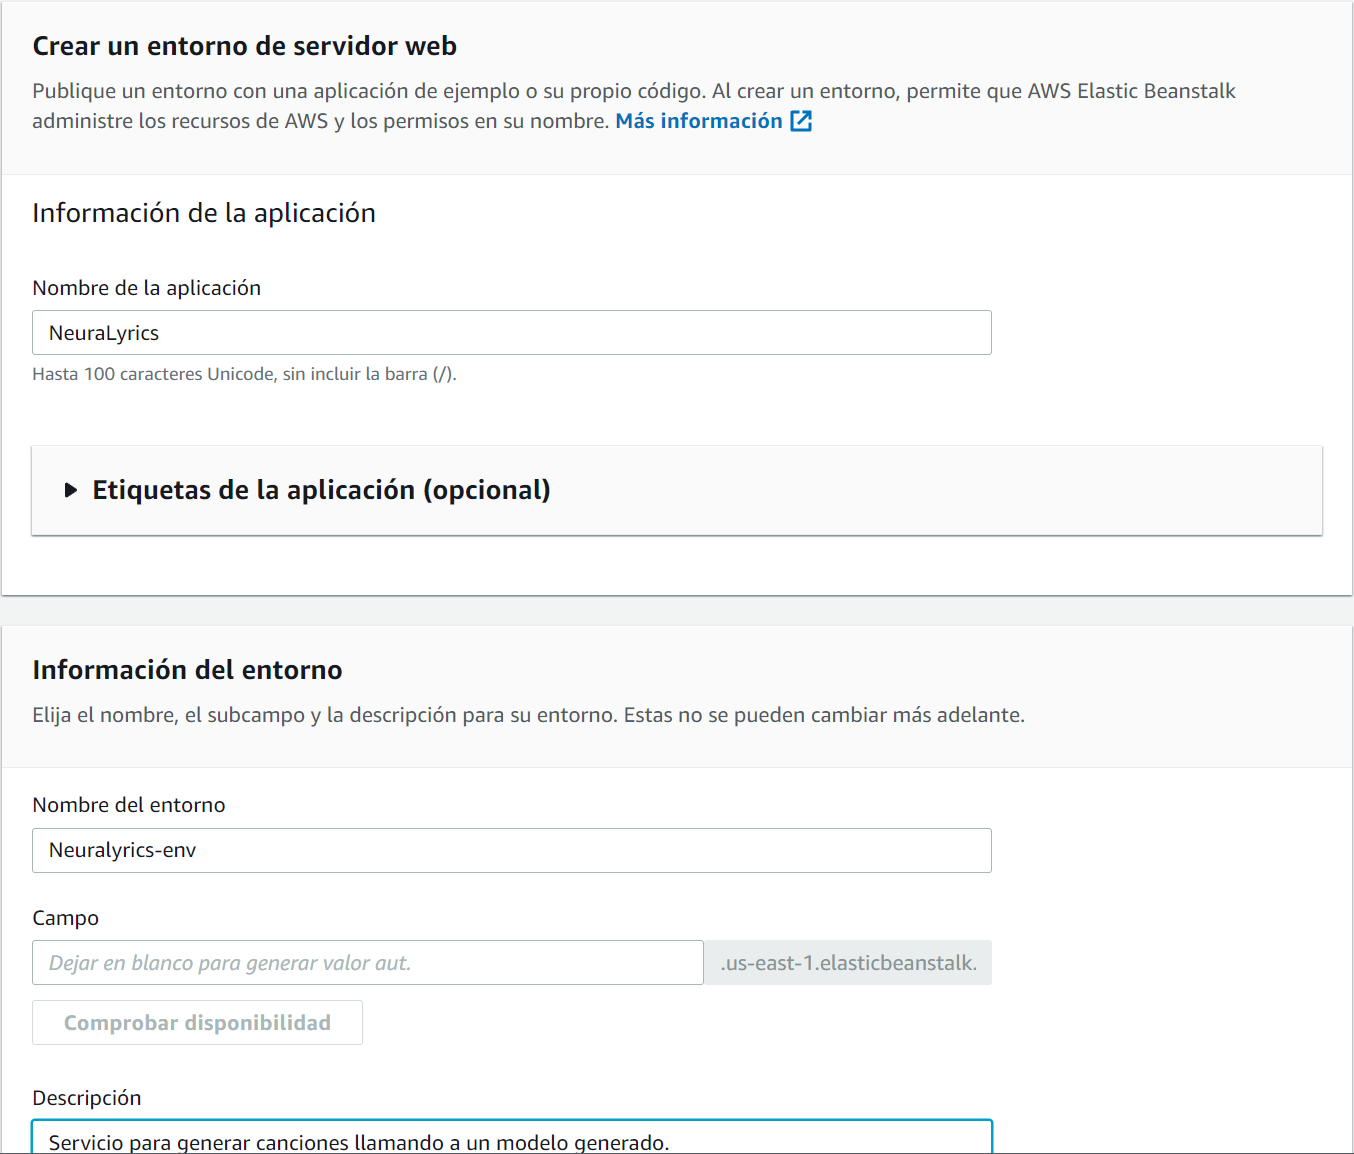
\includegraphics[width=12cm]{./Imagenes/BackEnd/paso_2.png}
			\centering 
			\caption{Crear un entorno de servidor.}
		\end{figure}
		Se elige el tipo de plataforma que se creará, en este caso se seleccionó como plataforma a Docker y se dejaron las configuraciones recomendadas por la misma plataforma.
		\begin{figure}[H]
			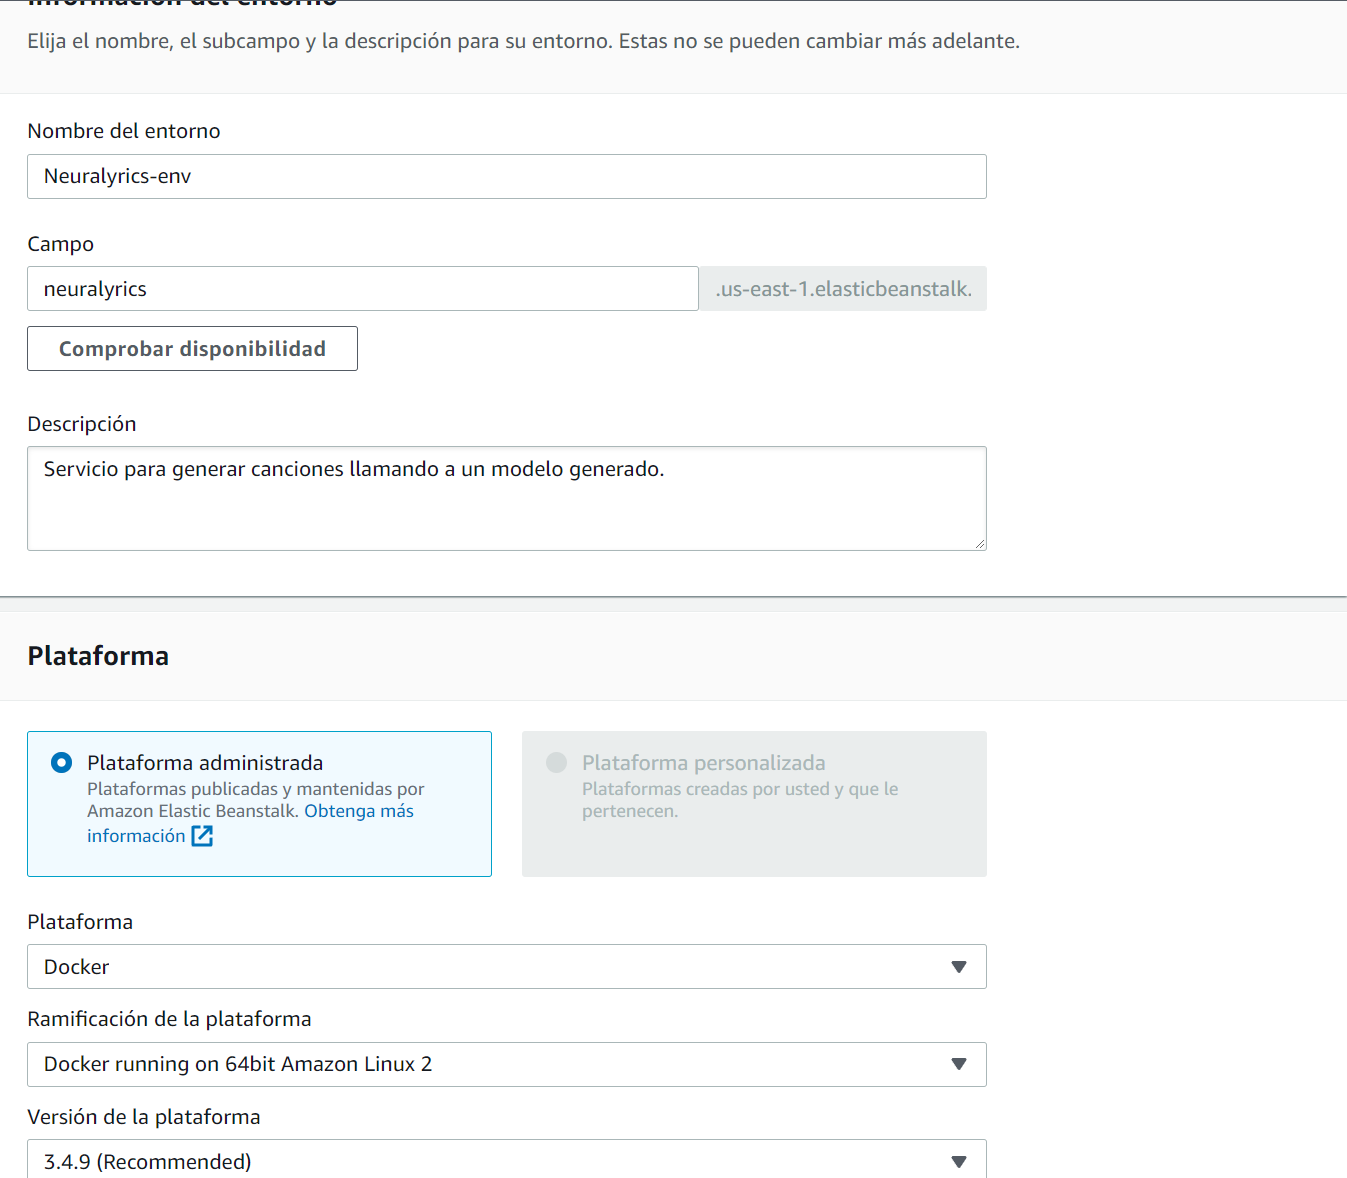
\includegraphics[width=12cm]{./Imagenes/BackEnd/paso_3.png}
			\centering 
			\caption{Elegir tipo de plataforma que utilizará el entorno.}
		\end{figure}
		Como último paso requerido para crear el entorno es necesario cargar el código en un bucket alojado en Amazon S3, siendo este el archivo con extensión .YML creado previamente, y así se pueda crear el entorno a partir de la imagen de Docker implementada previamente.
		\begin{figure}[H]
			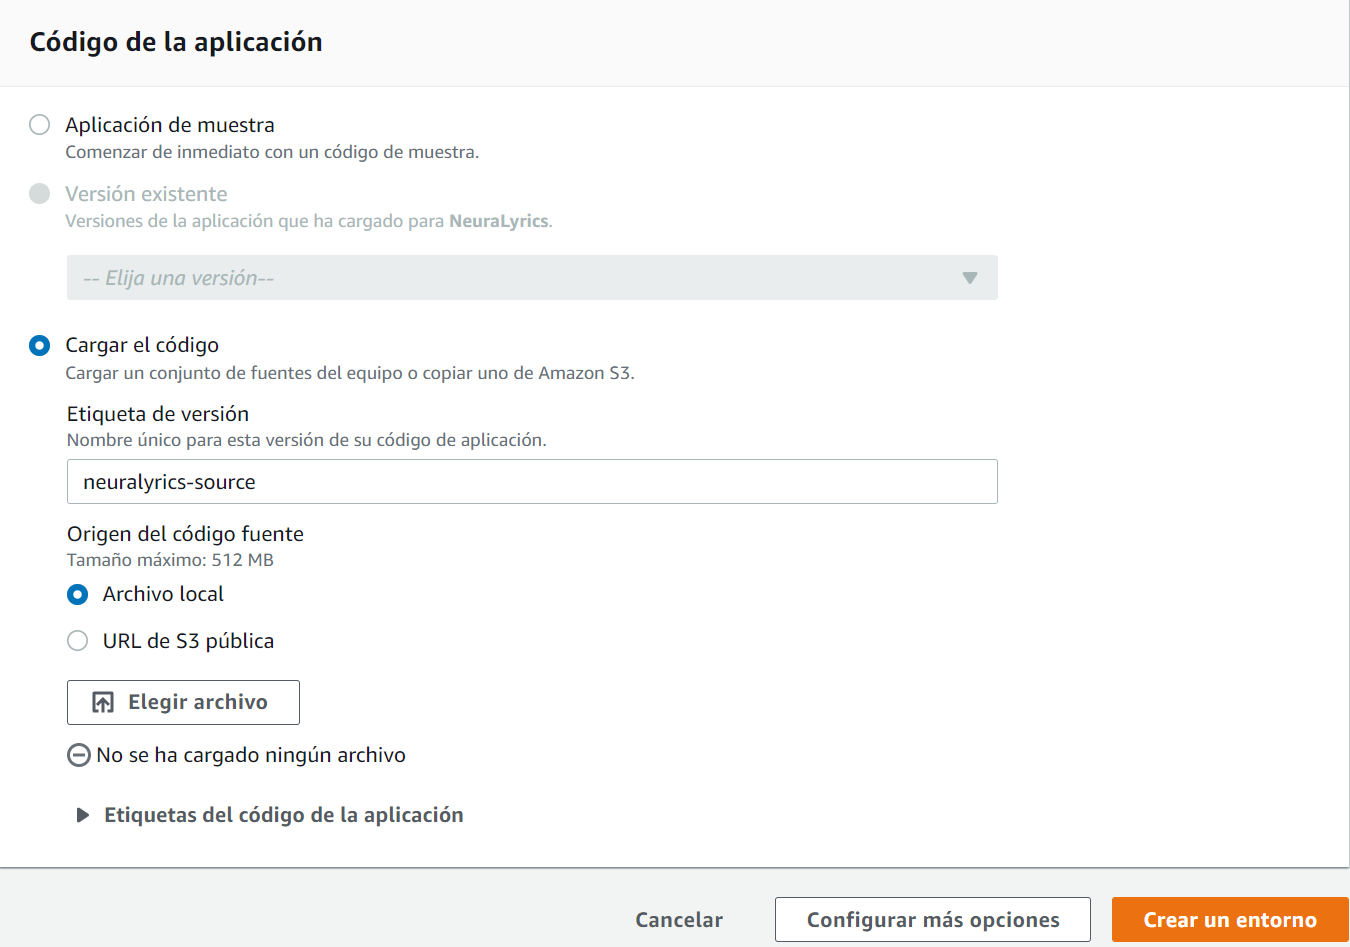
\includegraphics[width=12cm]{./Imagenes/BackEnd/paso_4.png}
			\centering 
			\caption{Subir el código de la aplicación.}
		\end{figure}
		Cuando se le da click al botón de crear entorno, se empezará a cargar la imagen y se debería mostrar el siguiente estado cuando se encuentre listo:
		\begin{figure}[H]
			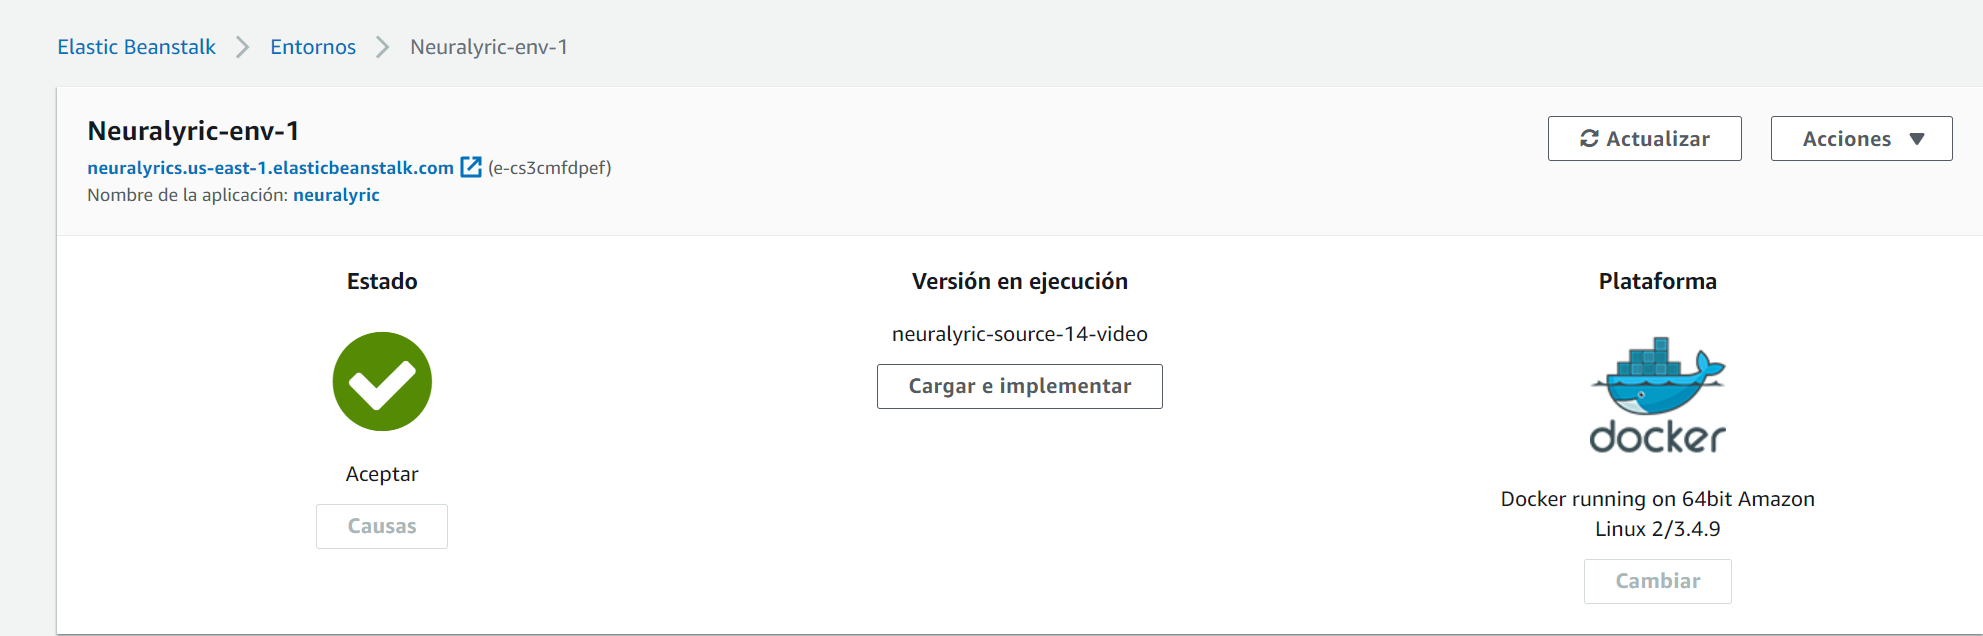
\includegraphics[width=12cm]{./Imagenes/BackEnd/paso_5.png}
			\centering 
			\caption{Despliegue del entorno.}
		\end{figure}
		Si todo salió bien en este punto ya se puede vislumbrar la API dentro del link generado, sin embargo, hay algunas configuraciones del entorno general (Fig. 25) que requieren unos cambios para que no haya ningún inconveniente al conectar el Front-end por medio de SSL.\\
		Es importante mencionar que se cambió manualmente el tipo de capacidad de “instancia individual” a “carga balanceada” con un mínimo de 1 y máximo de 1, esto no genera ningún cargo extra y permitirá configurar después y de manera correcta los certificados para escuchar al puerto 443 de SSL.
		\begin{figure}[H]
			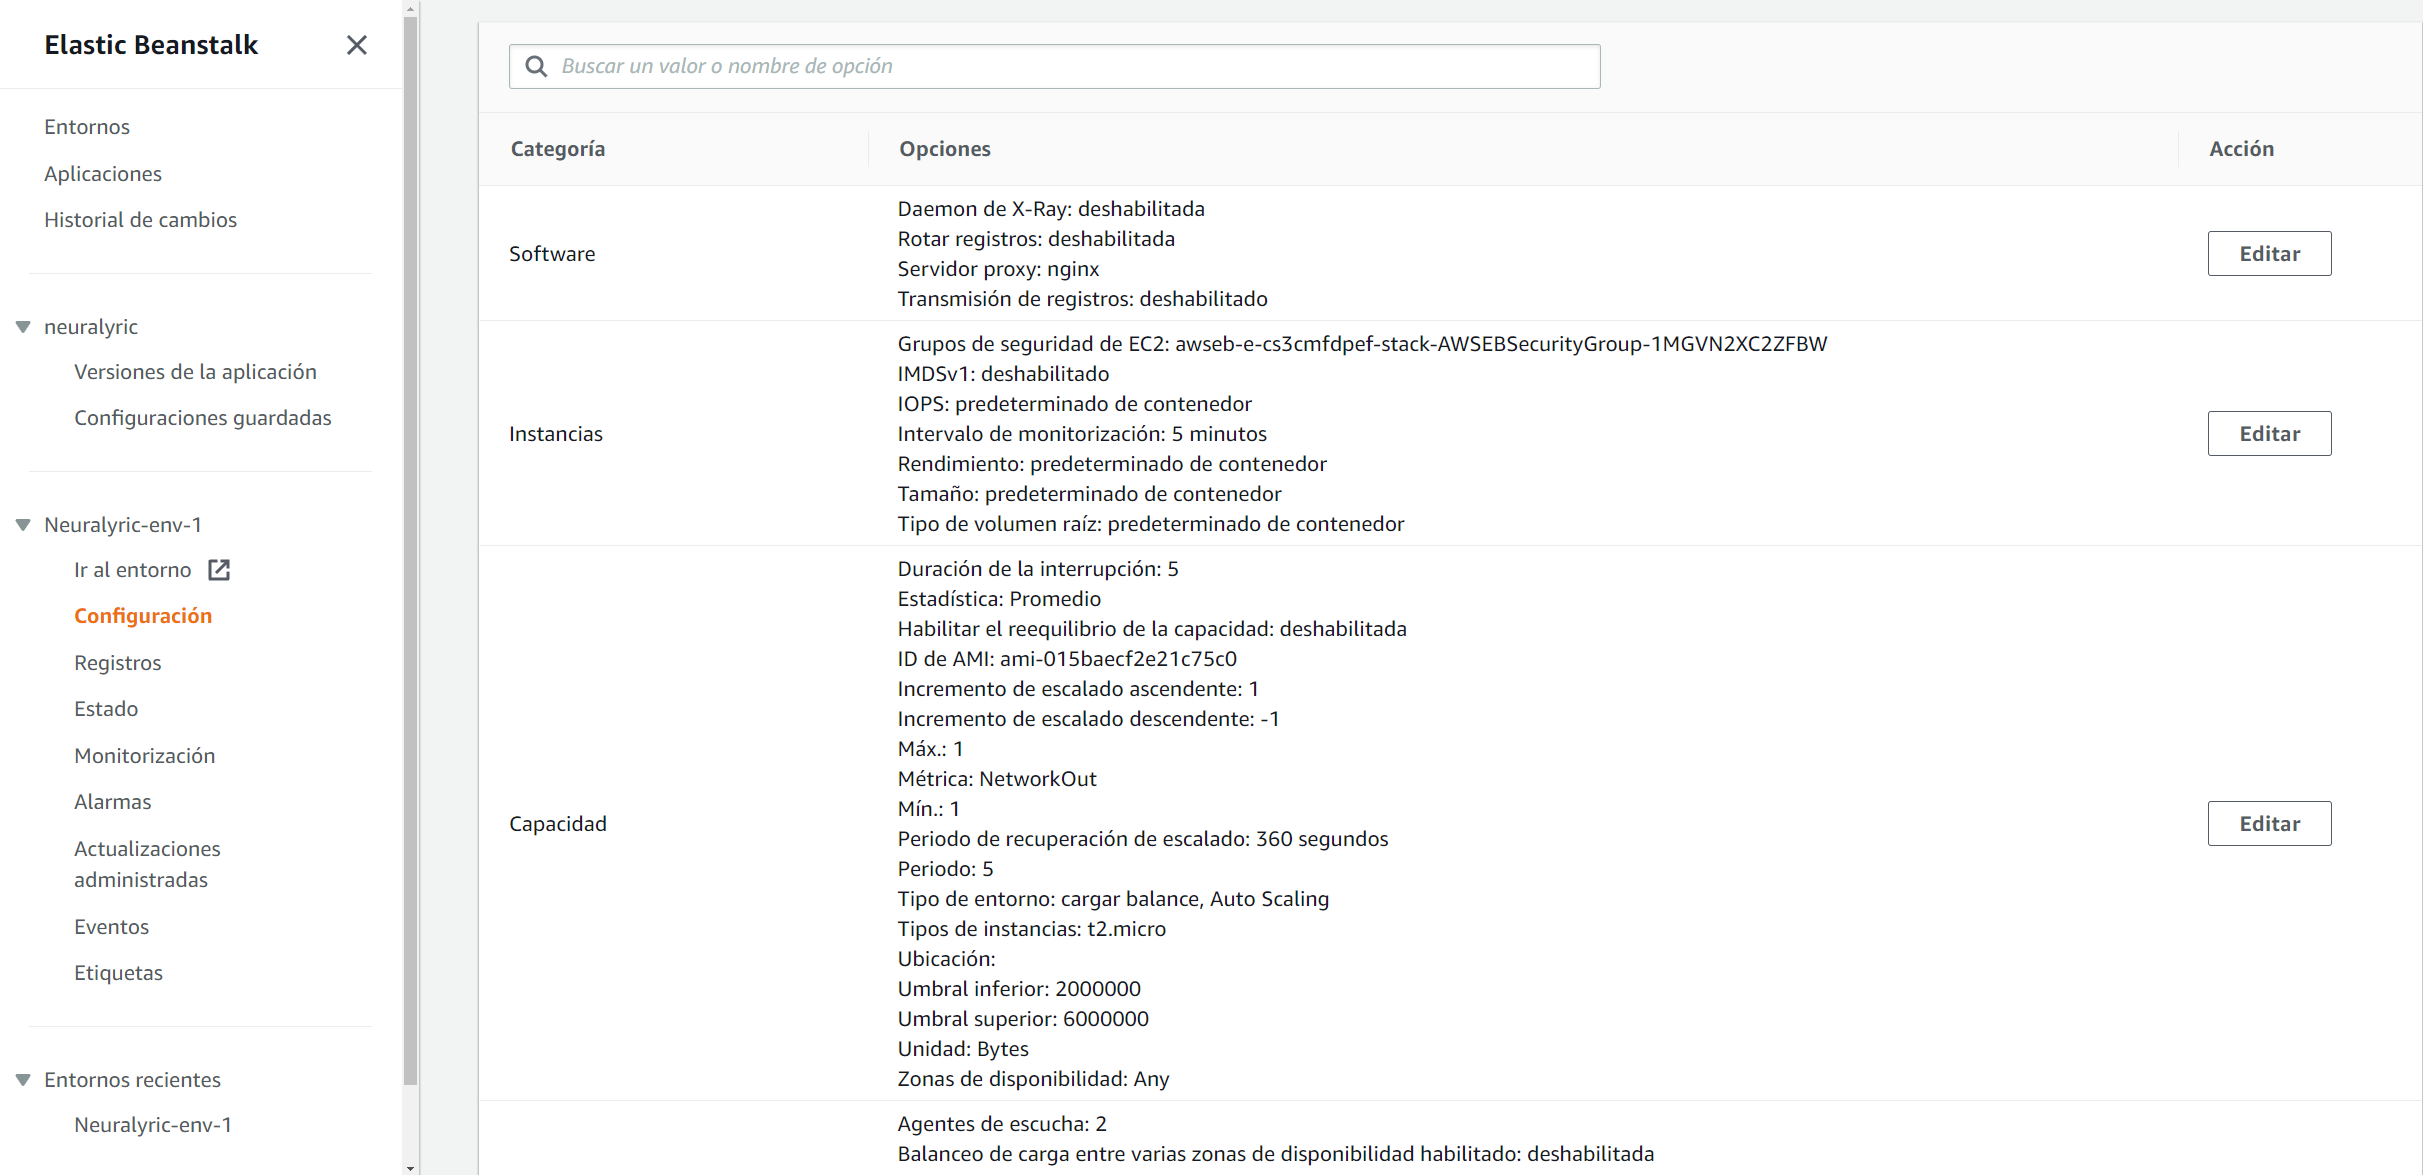
\includegraphics[width=12cm]{./Imagenes/BackEnd/config_1.png}
			\centering 
			\caption{Primera parte de las configuraciones generales de Elastic Beanstalk.}
		\end{figure}
		Continuando con las configuraciones requeridas, se cambió la configuración del balanceador de carga para que pueda redirigir los puertos de agente de escucha directamente a la API abriendo el puerto de SSL.
		\begin{figure}[H]
			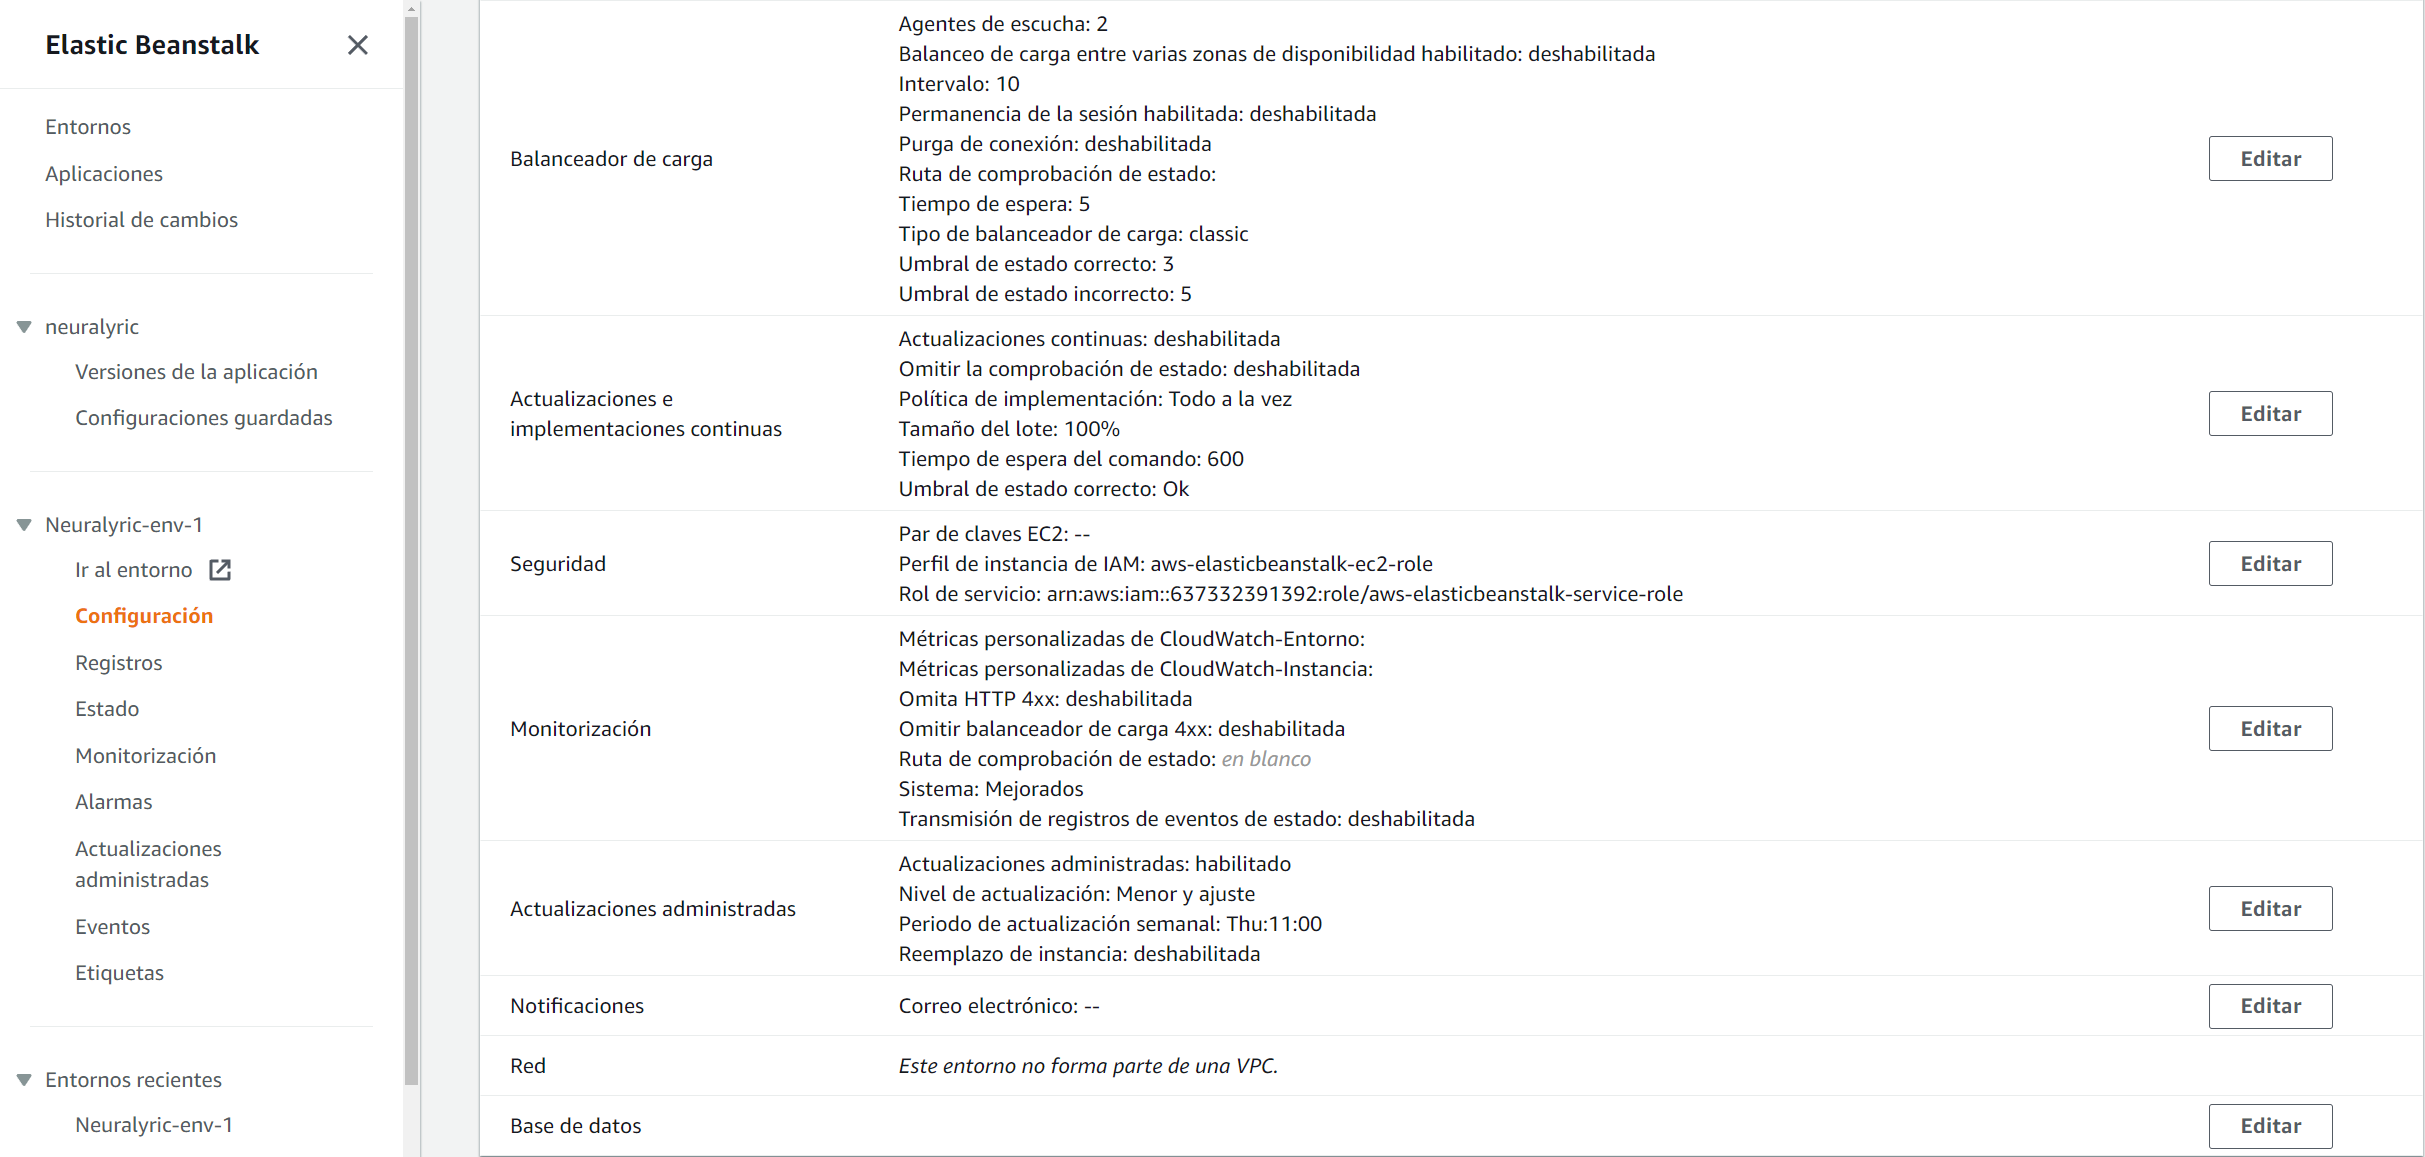
\includegraphics[width=12cm]{./Imagenes/BackEnd/config_2.png}
			\centering 
			\caption{Segunda parte de las configuraciones generales de Elastic Beanstalk.}
		\end{figure}
		\begin{figure}[H]
			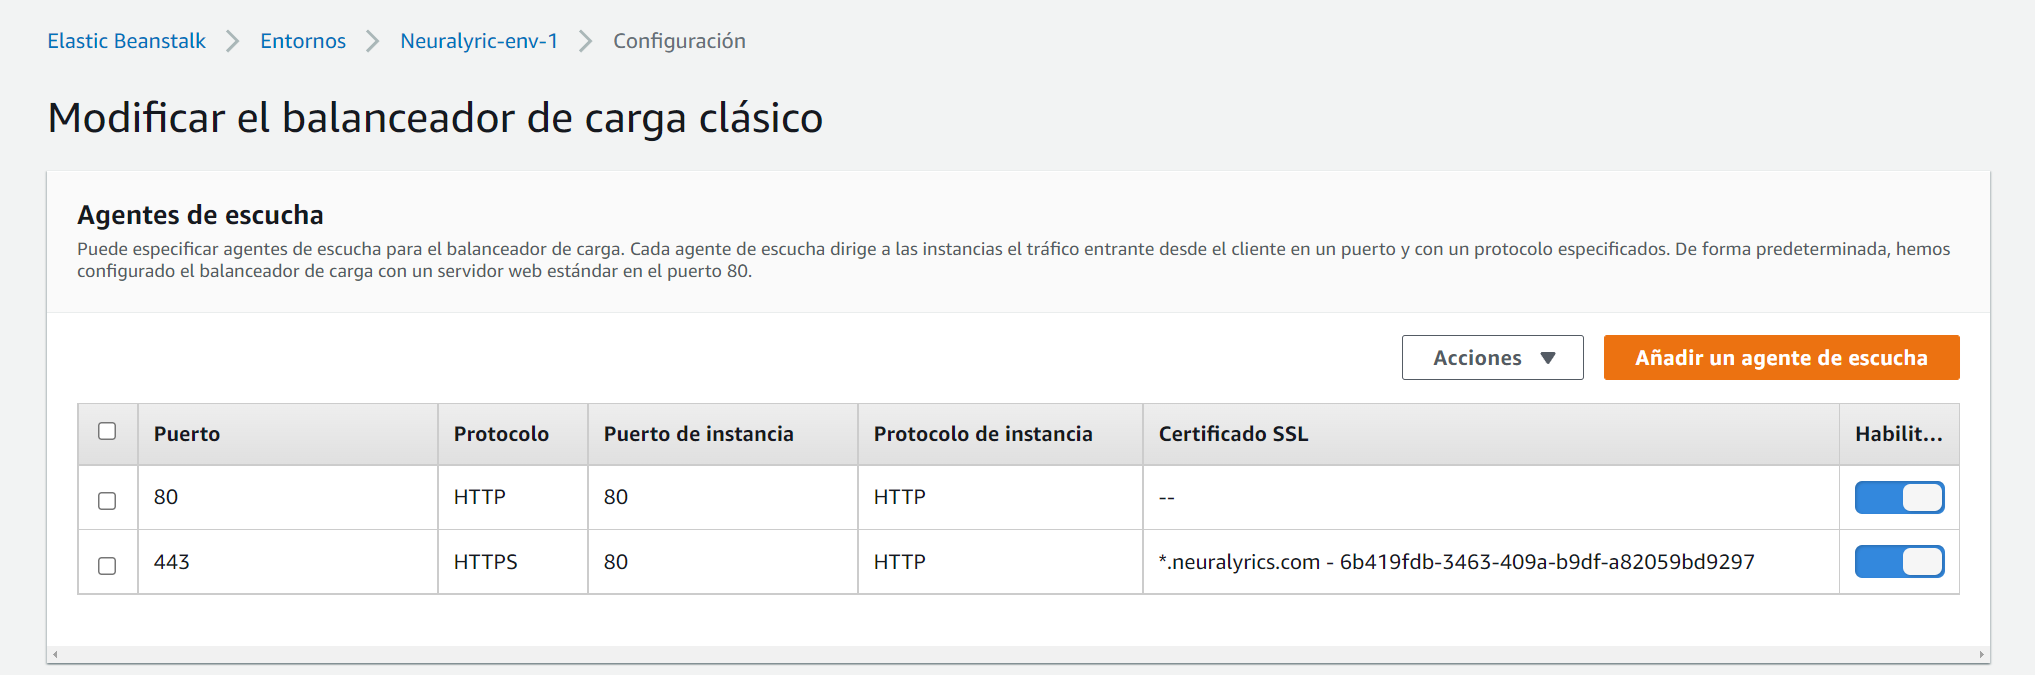
\includegraphics[width=12cm]{./Imagenes/BackEnd/config_balanceador.png}
			\centering 
			\caption{Despliegue del entorno.}
		\end{figure}
		Una vez configurado esto, se puede probar que la API este corriendo con los endpoints establecidos en el código de FLASK.
		\begin{figure}[H]
			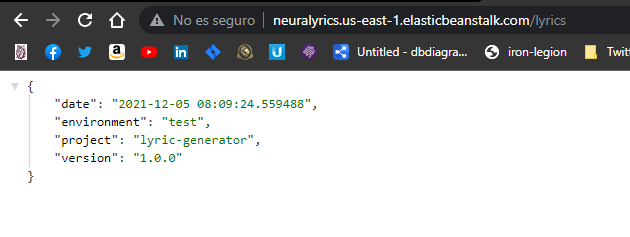
\includegraphics[width=12cm]{./Imagenes/BackEnd/api_corriendo.png}
			\centering 
			\caption{Estatus de la API corriendo con el endpoint configurado.}
		\end{figure}
		Una vez que la API se encuentre lista se recomienda hacer pruebas del funcionamiento total de la aplicación generada y checar los registros que arroja la plataforma de AWS, ya que cualquier error que la API pueda presentar en este punto puede afectar directamente a la página web, de igual forma se recomienda crear el certificado que aparece en la parte de “Configuración de SSL y DNS” para asegurar un correcto funcionamiento de la API usando HTTPS.
	\newpage
	\subsection{Despliegue de la página web}
	
	Para el despliegue de la pagina web nos apoyamos de la plataforma Vercel, la cual permite que los desarrolladores puedan desplegar sus paginas de manera rápida, así como poder actualizarla y escalarla de forma sencilla, además permite hacer despliegues de proyectos que se encuentren dentro de una cuenta de Github.\\\\
	Lo primero que se requiere hacer para poder trabajar con la línea de comandos de Vercel es instalarlo, para ello debemos recurrir a nuestra terminal y descargarlo usando el comando “npm i -g vercel” o “yarn global add vercel”.
	\begin{figure}[H]
		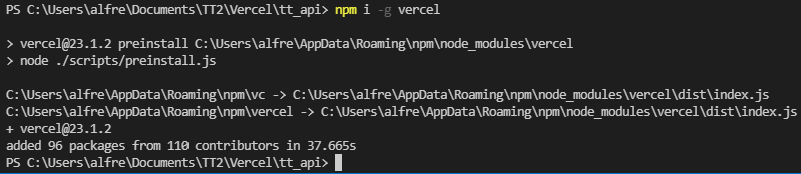
\includegraphics[width=12cm]{./Imagenes/Despliegue/Instalacion.png}
		\centering 
		\caption{Instalando CLI de Vercel}
	\end{figure}
	Una vez instalado, se debe de abrir la carpeta de nuestro proyecto a desplegar y abrir una terminal, es necesario escribir “vercel” para abrir el CLI de Vercel, el cual nos preguntará si el proyecto contenido dentro de la carpeta es el que se va a configurar y desplegar, posteriormente preguntará quien lo va a desplegar, para ello usamos una cuenta creada en la plataforma de Vercel o vinculamos la de Github para acceder, se nos pregunta el nombre del proyecto y el inicio de los archivos del proyecto a desplegar.
	\begin{figure}[H]
		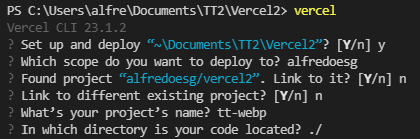
\includegraphics[width=12cm]{./Imagenes/Despliegue/Acciones.png}
		\centering 
		\caption{Indicando acciones para el despliegue}
	\end{figure}
	Una vez se configuraron las indicaciones anteriores, el CLI de Vercel detecta automáticamente el tipo de proyecto trabajado, en este caso una aplicación web usando React, y por último pregunta si se quiere cambiar la configuración del trabajo encontrado, en nuestro caso decimos que no, ya que es correcto el tipo de aplicación encontrada con el trabajado.
	\begin{figure}[H]
		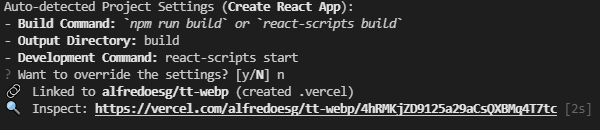
\includegraphics[width=12cm]{./Imagenes/Despliegue/Deteccion.png}
		\centering 
		\caption{Detección del tipo de proyecto a desplegar}
	\end{figure}
	Vercel comienza a desplegar la aplicación web y genera un enlace mediante el cual podemos ver el estado del despliegue, y de presentarse algún problema se nos estará indicando cual su origen en la misma terminal.
	\begin{figure}[H]
		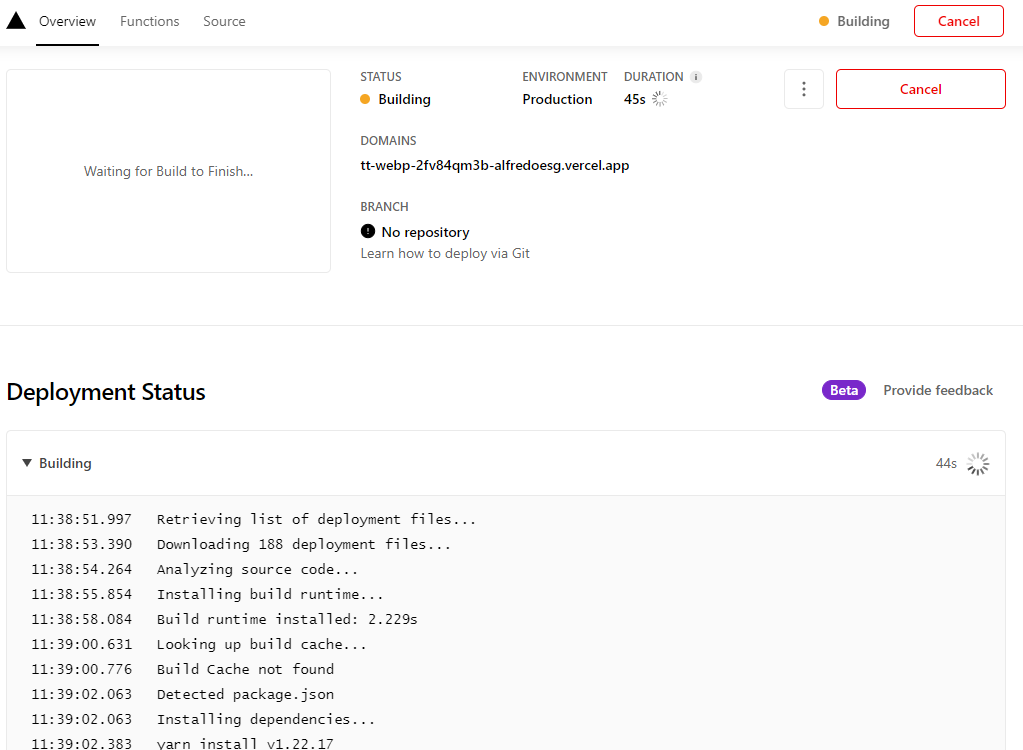
\includegraphics[width=12cm]{./Imagenes/Despliegue/Desplegando.png}
		\centering 
		\caption{Desplegando el proyecto}
	\end{figure}
	Al momento de desplegar la aplicación nos marca un error.
	\begin{figure}[H]
		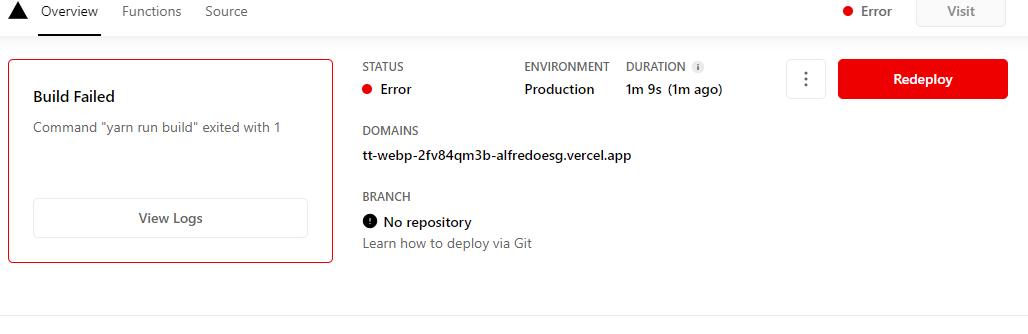
\includegraphics[width=12cm]{./Imagenes/Despliegue/Error.png}
		\centering 
		\caption{Desplegando el proyecto}
	\end{figure}
	Este error está relacionado con unas librerías opcionales localizadas dentro de la careta “node\_modules” de nuestro proyecto, Vercel no reconoce que estas librerías son opcionales por lo que para poder hacer el despliegue y que no nos marque error debemos entrar a las configuraciones de nuestro proyecto.	
	\begin{figure}[H]
		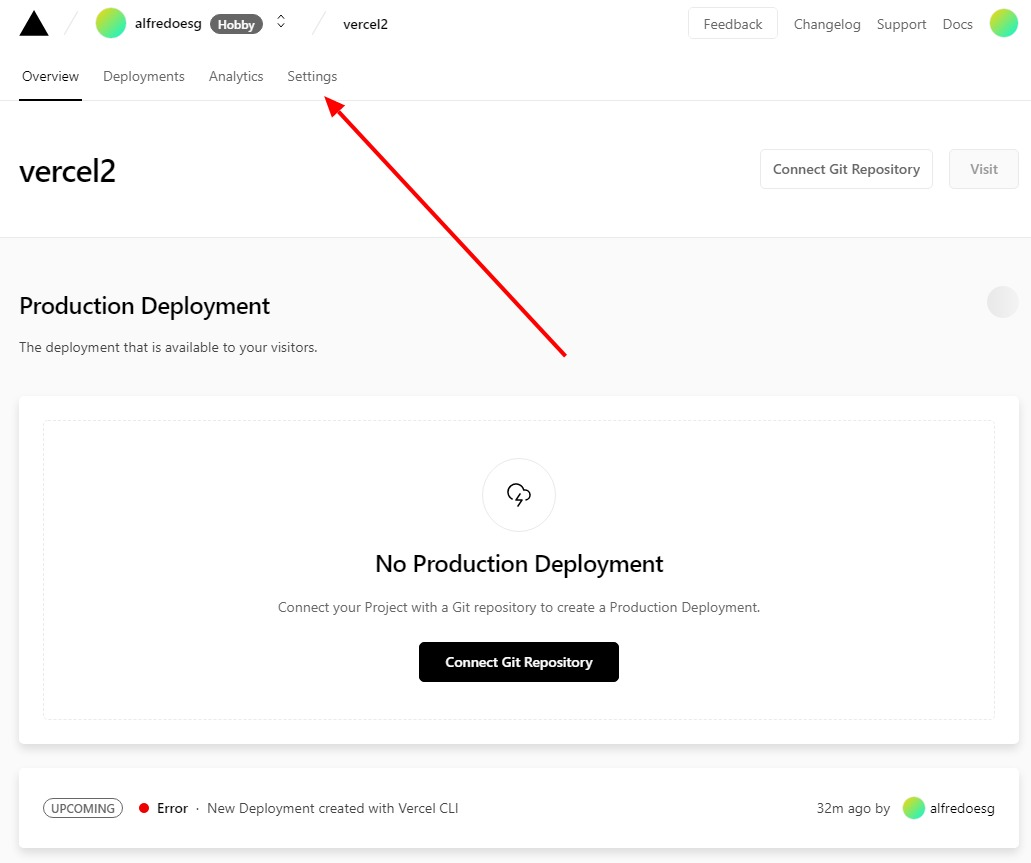
\includegraphics[width=12cm]{./Imagenes/Despliegue/Ajustes.jpeg}
		\centering 
		\caption{Configuración del proyecto desplegado}
	\end{figure}
	Una vez dentro de la configuración del proyecto se debe de ir a la sección de “variables de entorno” y ahí agregar la variable CI con un valor de false.
	\begin{figure}[H]
		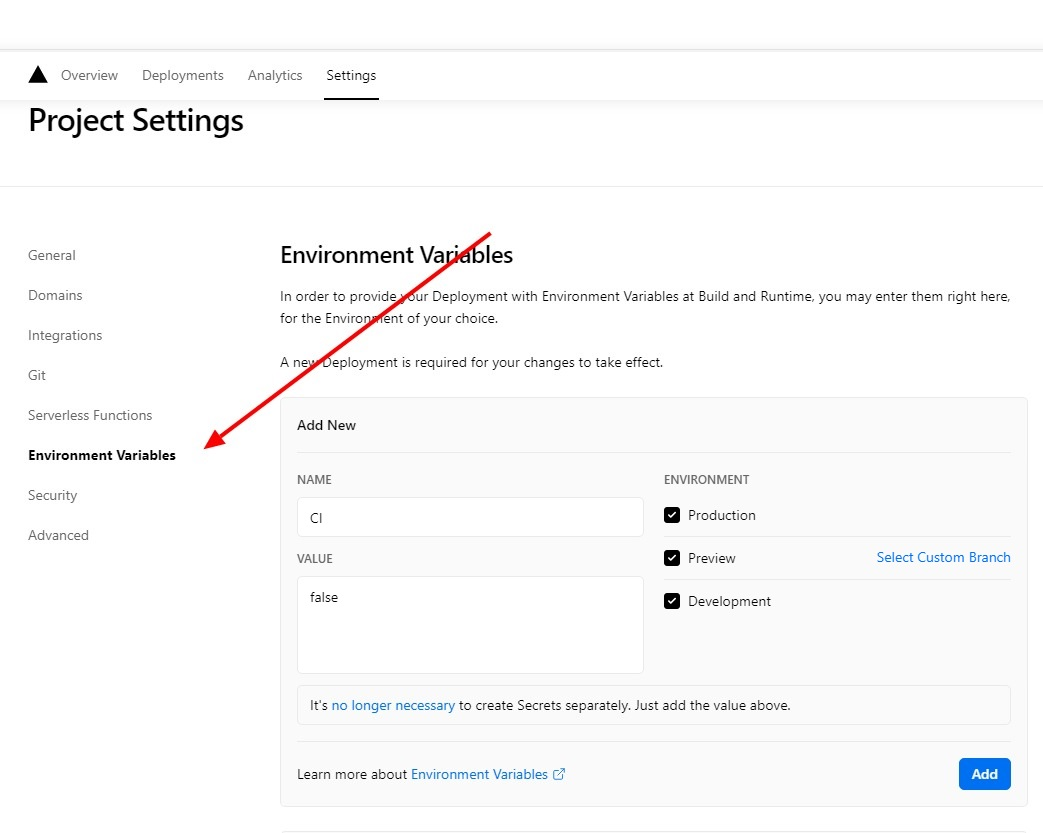
\includegraphics[width=12cm]{./Imagenes/Despliegue/Varaiblesentorno.jpeg}
		\centering 
		\caption{Variable de entorno}
	\end{figure}
	Habiendo realizado esos cambios se regresa a la terminal y se vuelve a escribir el comando “vercel” y automáticamente volverá a realizar el despliegue de la aplicación web. Con el comando vercel escrito en la terminal también es posible actualizar la página desplegada en caso de haber algún cambio en el código.\\\\
	Ya completado el despliegue se nos genera un enlace con el cual se puede acceder a la aplicación web desplegada desde cualquier dispositivo.
	\begin{figure}[H]
		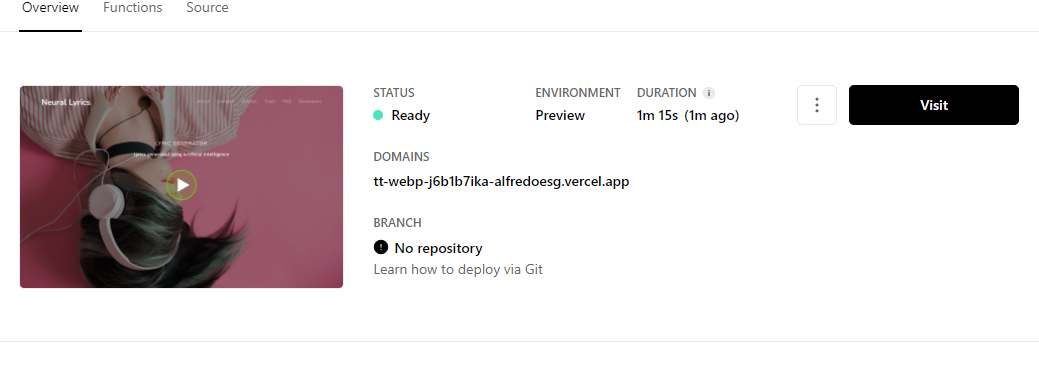
\includegraphics[width=12cm]{./Imagenes/Despliegue/Desplegada.png}
		\centering 
		\caption{Aplicación web desplegada}
	\end{figure}
	\begin{figure}[H]
		\includegraphics[width=12cm]{./Imagenes/Despliegue/Paginaweb.png}
		\centering 
		\caption{Accediendo a la aplicación web desplegada}
	\end{figure}
	En nuestro caso, previamente se había adquirido un dominio por lo que para realizar el cambio del enlace proporcionado por Vercel a el enlace del dominio adquirido hay que acceder nuevamente a la configuración del proyecto y ahí en la sección de “dominio” se agrega la nueva dirección desde la que queremos acceder.
	\newpage
	\section{Configuración de SSL y DNS}
	
	Para permitir que nuestra página web pueda accederse desde otros dispositivos es necesario hacer la configuración correcta de DNS y proporcionarle un certificado de seguridad. Dado que nuestra página web fue desplegada en la plataforma de Vercel, para que esta pueda direccionar de manera correcta usando nuestro dominio personal se requiere de la configuración de un DNS especifico requerido por Vercel.
	\begin{figure}[H] 
		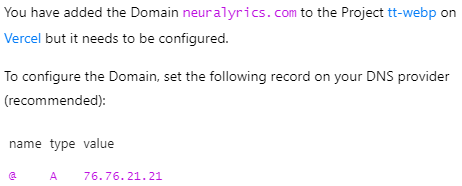
\includegraphics[width=10cm]{./Imagenes/DnsSSL/Dns1.png}
		\centering \caption{Dirección IP requerida para la configuración del DNS.}
	\end{figure}
	\begin{figure}[H] 
		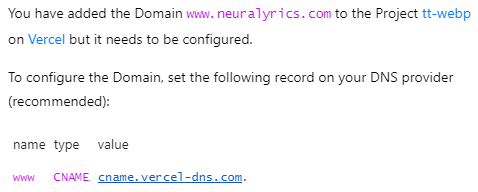
\includegraphics[width=10cm]{./Imagenes/DnsSSL/Dns2.png}
		\centering \caption{Nombre requerido para la configuración del DNS.}
	\end{figure}
	Por parte del backend se utilizó la herramienta gratuita de AWS Certificate Manager, la cuál nos permite agregar un certificado con el puerto número 443 abierto redirigiendo de HTTP a HTTPS, configurándolo para neuralyrics.com de manera que se pueda agregar un registro redireccionando a la API y no haya problemas de compatibilidad; una vez que la plataforma haya creado el certificado, se agregan dos registros a Cloudflare.
	
	\begin{figure}[H] 
		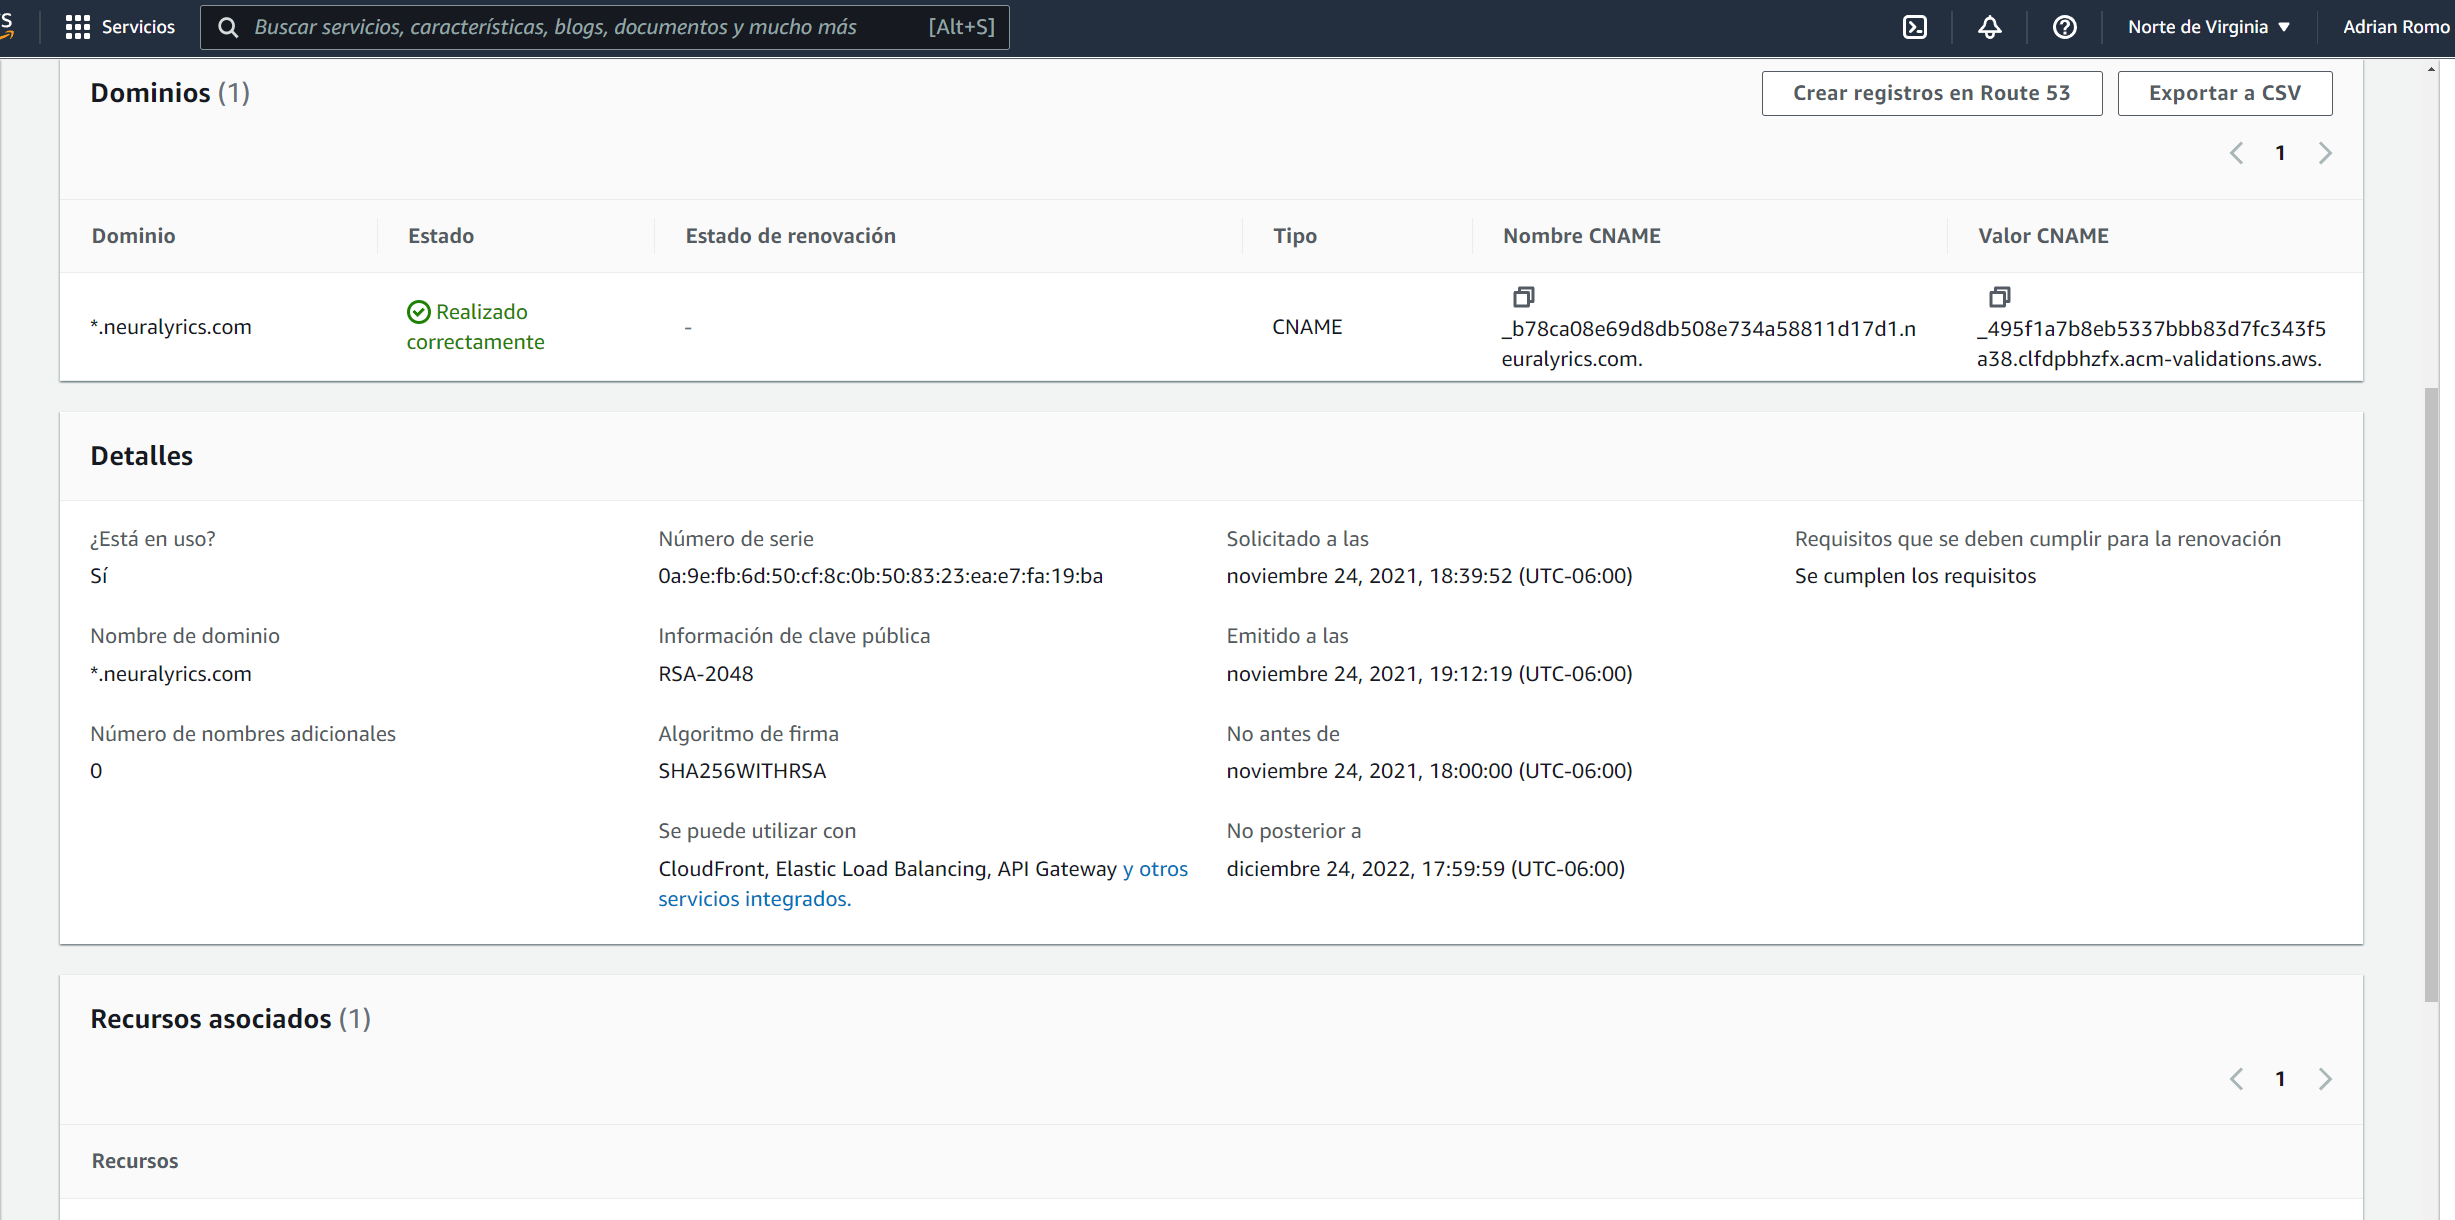
\includegraphics[width=10cm]{./Imagenes/DnsSSL/DNS_aws.png}
		\centering \caption{Estado del certificado SSL que se agregará en Cloudflare para que la API pueda funcionar con HTTPS.}
	\end{figure}
	Estas reglas de DNS deben agregarse en la plataforma de Cloudflare quedando de la siguiente manera.
	\begin{figure}[H] 
		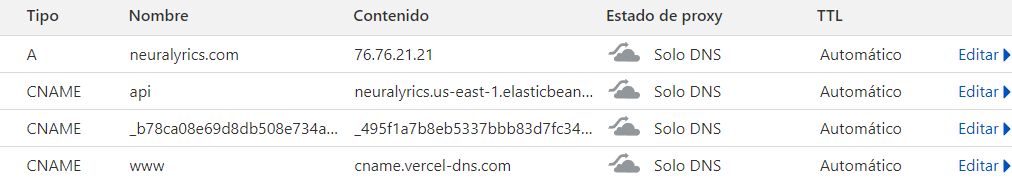
\includegraphics[width=10cm]{./Imagenes/DnsSSL/Config_DNS.png}
		\centering \caption{Configuración final de los registros DNS.}
	\end{figure}
	\begin{enumerate}
	\item El primero es la dirección de DNS proporcionado por Vercel de tipo, el cual permite enlazar una direccion con un nombre de dominio.
	\item El segundo es el código del certificado creado en AWS de tipo CNAME con el nombre y contenido proporcionado por AWS.
	\item El tercero es otro tipo CNAME con el nombre de “api” y conteniendo a la API directamente.
	\item El cuarto es el valor de tipo CNAME proporcionado por Vercel.
	\end{enumerate}
	Una vez desplegadas la página web y la API, y si todo se hizo correctamente, deberá ser posible comunicarse mediante los links generados al final de cada sección, cada parte tendrá su propio versionamiento, y una ventaja de esto es que pueden crecer los dos servicios de forma separada sin necesidad de depender de ellos, con lo que si una incurre en un error no deberá afectar el acceso al enlace de la otra.
	\newpage
		\begin{thebibliography}{20}
			\bibitem{refQuesPython} 
			Python (2021), What is Python? Executive Summary, [En línea]. Disponible: https://www.python.org/doc/essays/blurb/ [Último acceso: 24 de abril del 2021].
			\bibitem{refHtml}
			Mozilla.org (2021, febrero 19), HTML basics, [En línea]. Disponible: https://developer.mozilla.org/en-US/docs/Learn/Getting\_started\_with\_the\_web/HTML\_basics [Último acceso: 15 de mayo del 2021].
			\bibitem{refHtml2}
			Mozilla.org (2021, mayo 14), HTML5, [En línea]. Disponible: https://developer.mozilla.org/es/docs/Web/Guide/HTML/HTML5 [Último acceso: 15 de mayo del 2021].
			\bibitem{refcss}
			W3C (2016), HTML \& CSS, [En línea]. Disponible: [Último acceso: 15 de mayo del 2021].		
			\bibitem{refjs}
			Mozilla.org (2021, abril 27), What is JavaScript?, [En línea]. Disponible: https://developer.mozilla.org/en-US/docs/Learn/JavaScript/First\_steps/What\_is\_JavaScript [Último acceso: 15 de mayo del 2021].
			\bibitem{amazon_ec2}
			Amazon (2021), Amazon EC2 [En línea]. Disponible: https://aws.amazon.com/es/ec2/?ec2-whats-new.sort-by=item.additionalFields.postDateTime\&ec2-whats-new.sort-order=desc [Último acceso: 1 Junio 2021]
			\bibitem{amazon_elastic_beanstalk}
			Services, A. (2021). Introducción a AWS Elastic Beanstalk. Amazon Web Services, Inc. https://aws.amazon.com/es/elasticbeanstalk/ [Último acceso: 1 Junio 2021]
			\bibitem{amazon_s3}
			Amazon (2021), Amazon S3 [En línea]. Disponible: https://aws.amazon.com/es/s3/ [Último acceso: 1 Junio 2021]		
			\bibitem{kaggle}
			Kaggle (2010), How to Use Kaggle [En línea]. Disponible: https://www.kaggle.com/docs/datasets [Último acceso: 25 Mayo 2021]
			\bibitem{kaggleDataset}
			Kaggle (2019, Noviembre 17), Song lyrics from 6 musical genres [En línea]. Disponible: https://www.kaggle.com/neisse/scrapped-lyrics-from-6-genres [Último acceso: 25 Mayo 2021]
			\bibitem{vagalume}
			Vagalume (2002), Vagalume: Music e tudo [En línea]. Disponible: https://www.vagalume.com.br/ [Último acceso: 25 Mayo 2021]		
			\bibitem{data_cleaning}
			Aaron Tay (2021, Abril 23), Data Cleaning Techniques [En línea]. Disponible: https://www.digitalvidya.com/blog/data-cleaning-techniques/ [Último acceso: 30 Mayo 2021]
			\bibitem{tokenimagen}
			B. Lee (2019, Noviembre 17), How to 10x Response Rates on Surveys [En línea]. Disponible: https://bryankmlee3.medium.com/conducting-surveys-with-nlp-d38df4c29e39 [Último acceso: 5 Junio 2021]
			
		\end{thebibliography}	
	\end{document}